%%%%%%%%%%%%%%%%%%%%%%%%%%%%%%%%%%%%%%%%%%%%%%%%%%%%%%%%%%%%%%%%%%%%%%%%%%%%%%%%
\chapter{Modeling and Algorithms}\label{ch:modeling-evaluation}
%%%%%%%%%%%%%%%%%%%%%%%%%%%%%%%%%%%%%%%%%%%%%%%%%%%%%%%%%%%%%%%%%%%%%%%%%%%%%%%%


%%%%%%%%%%%%%%%%%%%%%%%%%%%%%%%%%%%%%%%%%%%%%%%%%%%%%%%%%%%%%%%%%%%%%%%%%%%%%%%%
\section{Introduction}


This chapter describes in-depth the implementation of the traffic modeling algorithms mentioned in Chapter 3. The first section gives a brief survey of other works that presented methodologies for a parameterizing stochastic process to describe internet traffic (inter-packet times and packet-trains). This introduction shows a scenario where there is no "one-fits-all" model. The best model always depends on the type of traffic. 

Many consolidate works investigate the nature of internet traffic, and many others on the modeling of stochastic functions for specific scenarios. However, there are not as many on model choice automation. In the second section, we discuss and cross-validate our methodology for automating the choice of inter-packet times processes. We select inter-packet times models using information criteria ($AIC$ and $BIC$) to rank the models from the best to the worst.  Since, to the best of our knowledge, there was no previous validation of the effectiveness of $AIC$ and BIC for ranking information criteria, we developed our cross-validation methodology to test their effectiveness.  

In the third section, we present our algorithm called "\texttt{calcOnOff}", a method to estimate packet trains periods (ON and OFF times) of an arbitrary flow, which do not rely on header fields, but just times between packets. Finally, the fourth section shows our strategy for guessing application protocols from flows, protocols using common transport header fields.


We use refer to two different cost functions on this chapter. The first is the Gadient Descendent Cost function, we refer as $J_\nabla$, since nabla ($\nabla$) is the notation used to represent gradients. The second is our cross-validation cost function, we refer as $J_M$, since it is used to rank stochastic models ($M$).


%%%%%%%%%%%%%%%%%%%%%%%%%%%%%%%%%%%%%%%%%%%%%%%%%%%%%%%%%%%%%%%%%%%%%%%%%%%%%%%%
\section{Literature Review on internet traffic modeling}


There are many works devoted to studying the nature of the Ethernet traffic\cite{selfsimilar-ethernet}. Classic Ethernet models used Poisson related processes to model traffic\footnote{In our study case we used two Poisson related processes, both using exponential distributions: Exponential(Me) and Exponential(LR). Exponential distributions are considered continuous versions of the Poisson process.  Since we are using time as a real number, we preferred to use just exponential distributions, for simplicity.}. A Poisson process represents the probability of events occur with a known average rate, and independently of the last occurrence\cite{book-poisson}. 

However, studies made by Leland et al.  showed that the Ethernet traffic has a self-similar and fractal nature. Even if they can represent the randomness of   Ethernet traffic, simple Poisson processes cannot express traffic "burstiness" on a long-term timescale, such as traffic "spikes" on long-range "ripples". These characteristics are an indication of the fractal and self-similar nature of the traffic, that usually we express by distributions with infinite variance, called heavy-tailed. Heavy-tail means that a stochastic distribution is not exponentially bounded\cite{sourcesonoff-paper}, and can guarantee self-similarity via Joseph and Noah effects\cite{selfsimilar-highvariability}. Examples of heavy-tailed functions are Weibull, Pareto, Cauchy. However, these distributions may guarantee self-similarity, but not necessarily they will ensure other features like good correlation and same average packet rate\cite{validate-trafficgen}. 

There are plenty of works in the literature which proposes processes and methodologies for modeling times between packets and packet trains\cite{selfsimilar-ethernet}\cite{analysis-self-similar}\cite{stochastic-selfsimilar}\cite{selfsimilar-highvariability}\cite{multi-player-online-game-self-similarity}\cite{estimation-renewal-function-ethernet-traffic}\cite{modelling-of-self-similar}\cite{empirical-interarrival-study}\cite{modeling-concurrent-heavy-tailed}\cite{optimal-scheduling-of-heavy-tailed-traffic}\cite{modelling-of-self-similar}. Fiorini\cite{modeling-concurrent-heavy-tailed}  presented a heavy-tailed ON/OFF model, which represented the traffic generated by many sources. The model emulated a multiple source power-tail Markov-Modulated (\acrshort{PT-MMPP}) ON/OFF process, where the ON times have been power-tail distributed. They achieve analytical performance measurements using Linear Algebra Queueing Theory. 

Kreban and Clearwater\cite{hierarchical-dynamics-interarrival-times}  presented a model for times between job submissions from multiple users over a supercomputer. They have shown that the Weibull probability functions can express well small and high values of inter-job submission times. They also have tested exponential, lognormal and Pareto distributions. The Exponential distribution has not represented well long-range values because of it had felt-off too fast. On the other hand, the Pareto problem was that it had felt too slow. Lognormal have fitted well small values, but its performance had been weak on larger ones. Kronewitter\cite{optimal-scheduling-of-heavy-tailed-traffic} has presented a model of scheduling traffic of many heavy-tail sources. On his work, he had used many Pareto sources to represent the traffic. To estimate Pareto shape (parameter $\alpha$) he had used linear regression.


%%%%%%%%%%%%%%%%%%%%%%%%%%%%%%%%%%%%%%%%%%%%%%%%%%%%%%%%%%%%%%%%%%%%%%%%%%%%%%%%
\section{Automatized selection of inter-packet times models using \textit{AIC} and \textit{BIC}}

\subsection{Cross-validation Methodology}

There many consolidate works which have investigated the nature of internet traffic, and many others that had proposed processes to describe network traffic on specific scenarios. But not as many on model choice automation.  We propose and evaluate the use of the information criteria $BIC$ (Bayesian Information Criterion) and $AIC$ (Akaike Information Criterion) as suitable methods for automated model selection for inter-packet times.  

We then define our cross-validation method based on a cost function $J_M$,  which is an aggregator of traditional and critical metrics used on validation of stochastic models and traffic generators: Correlation(quality of the model), Average inter packet-time (related with the traffic Throughput), and Hurst Exponent (traffic fractal level).  $J_M$ assign weights from the best to the worst representation for each property of each trace model by using randomly generated data with our stochastic fittings. Through this process, we choose the best-fitted traffic model under evaluation. Afterward, we compare the results achieved by $AIC$/$BIC$ and our cost function. Given the approach mentioned above, we show that $AIC$/$BIC$ methods provide an intelligent stochastic process selection strategy for inter-packet times models.
We summarize the validation process in the steps below:
\begin{enumerate}
\item We have selected many \textit{pcap} files, representing different types of network scenarios. We extracted from these files the list of inter-packet times.
\item Using a set of stochastic functions, and parameterization methods, we defined a list of candidate stochastic processes to represent the inter-packet time's distribution for each dataset.
\item For each dataset, $AIC$ and $BIC$  were used to rank the processes, from the best to the worst, for each dataset.
\item Using each process from step four,  we generated random data and estimated the cost function $J$. We have repeated the random data generation  30 times, and the parameters used on the cost function had ion had a confidence interval of 95\%. Finally, we have ranked the processes from the best to the worst for each dataset.
\item Finally, we had two independent rankings, the one we wanted to validate, and others based on the literature. We compared the results.
\end{enumerate}
  
We also present some \textit{QQplots}, to visually compare the random-generated data and the original data-set. 


\subsection{Datasets}


We will use four \textit{pcap} files, where three are publicly available, to enable the reproduction of the simulations described in this chapter. The first is a lightweight Skype capture, found in Wireshark wiki 2, located at https://wiki.wireshark.org/Samp\footnote{https://wiki.wireshark.org/}, located  at \href{https://wiki.wireshark.org/SampleCaptures}{https://wiki.wireshark.org/SampleCaptures}. The file name is \texttt{SkypeIRC.cap}. We will call this trace \textit{skype-pcap}. The second is a CAIDA\footnote{http://www.caida.org/home/}{http://www.caida.org/home/} capture, and we can found it at \href{https://data.caida.org/datasets/passive-2016/equinix-chicago/20160121-130000.UTC}{https://data.caida.org/datasets/passive-2016/equinix-chicago/20160121-130000.UTC}. Access to this file requires a login, so is required the creation and approval of a new account.  The pcap's file name is \texttt{equinix-chicago.dirB.20160121-135641.UTC.anon.pcap.gz}. We call it \textit{wan-pcap}\footnote{\acrshort{WAN} stands for Wide Area Network}.

The third we capture in our laboratory \acrshort{LAN}, through a period of 1 hour in a firewall gateway between our local and external network. We call it \textit{lan-firewall-pcap}. The fourth is a capture of a busy private network access point to the Internet, available online on TCPreplay website\footnote{ \href{http://tcpreplay.appneta.com/wiki/captures.html}{http://tcpreplay.appneta.com/wiki/captures.html}}, called \texttt{bigFlows.pcap}. We will refer to it \textit{lan-gateway-pcap}.

We retrieved inter-packet times from the traffic traces and divided them into two equally sized datasets. We split the data based on the index of the array we use to store. Odd-indexed elements have been used as a training dataset, and even-indexed for cross-validation; to avoid data over-fitting.


\subsection{Stochastic Processes Modeling and Selection}


\subsubsection{Stochastic Processes}

We have adopted five stochastic functions (\textbf{Weibull}, \textbf{Normal}, \textbf{Exponential}, \textbf{Pareto} and \textbf{Cauchy}), and three methods for parameters estimation: \textbf{Linear Regression}, \textbf{Direct estimation}, and \textbf{Maximum Likelihood}, totaling seven stochastic processes : 
\begin{enumerate}
\item \textbf{Weibull} via Linear Regression;
\item \textbf{Normal} via Direct Estimation;
\item Exponential via Direct Estimation, we refer as \textbf{Exponential(LR)};
\item Exponential via Linear Regression, we refer as \textbf{Exponential(MLH)};
\item Pareto via Linear Regression, we refer as \textbf{Pareto(LR)};
\item Pareto via Maximum Likelihood, we refer as \textbf{Pareto(MLH)};
\item \textbf{Cauchy} via Linear Regression.
\end{enumerate}



The data that have been used for modeling was the training dataset. $AIC$, $BIC$ and the cost function have used the cross-validation dataset. Since the time samples resolution used were of $10^{-6}$s, all values equal to zero had been set to $5\cdot10^{-8}$s, to avoid division by zero. To avoid divergence in tangent operation used  Cauchy linearization process, we have floor-limited and upper-limited the inter-packet CDF values by  $10^{-6}$ and $0.999999$, respectively. We implemented this prototype using Octave and Python. We upload all the code and data from these experiments on Github\cite{aic-bic-repo}. 


\subsubsection{Linear regression (Gradient descendant)}


Linear regression is a method for estimating the best linear curve in the format:

\begin{equation}
y = ax + b
\end{equation}

to fit a given data set. We can use linear regression to estimate parameters of a non-linear curve expressing it on a linear format. For example, the Weibull CDF for $t > 0$ is:

\begin{equation}
F(t|\alpha, \beta) = F(t) = 1 - e^{-(t/\beta)^{\alpha}}
\end{equation}

Manipulating the equation:

\begin{equation}
\alpha\ln{(t)} - \alpha\ln{(\beta)} = \ln{(-\ln{(1 - F(t))})}
\end{equation}

If we call $x = \ln{(t)}$ and $y = \ln{(-\ln{(1 - F(t))})}$, we found a linear equation, where  $a = \alpha$ and $b = -\alpha\ln{(\beta)}$. Having in hands an estimation of the empirical CDF of our data samples, we apply the $x$ and $y$ definitions to linearize the data.

Using the gradient descendant, we find an estimation of the linear coefficients: $\hat{a}$ and  $\hat{b}$.  Using the inverse function of linear factors, we see the Weibull estimated parameters  $\hat{\alpha}$ and $\hat{\beta}$.

\begin{equation}
\alpha = a
\end{equation}

\begin{equation}
\beta = e^{-(b/a)}
\end{equation}


The gradient descendent consists of minimizing a cost function $J_\nabla(\theta)$, whose value decrease if the approximation becomes better. We explain this procedure in the appendix ~\ref{ap:revision-probability}. In the figure~\ref{fig:linearization} we present as examples, the linearized data for the inter arrivals from the \textit{skype-pcap}, and in the figure~\ref{fig:cost} the cost convergence. Appendix ~\ref{ap:aditional-plots} presents a complete set of figures.

Applying the inverse equations of the linear coefficients ($\hat{\alpha} = \hat{a}$ and $\hat{\beta} = e^{-(\hat{b}/\hat{a})}$  \footnote{We use the hat symbol ( $ \widehat{} $ ) for estimated parameters}, we can estimate the Weibull distribution parameters. We can summarize this procedure, in these steps:

\begin{enumerate}
\item Linearize the stochastic CDF function $F(t)$.
\item Apply the linearized  $y = y(F(t))$ and $x = x(t)$ on the empirical CDF and times datasets, respectively.
\item Use Gradient Descendant algorithm to find linear coefficients a and b.
\item Apply the inverse equation of the linear coefficients, to determine the stochastic function parameters.
\end{enumerate}



In the parameters estimation (step 4), there is an exception, since the Pareto scale ($x_{m}$) is defined by the smaller time allowed. In table~\ref{tab:linearization-sumary} we present a summary of the used equations in the procedure. In this notation, the subscript $i$ means that it is applied to every value measured empirically.


\begin{table}[h!]
    \centering
    \caption{Linearized functions, and parameters estimators, used by the linear regression}
    \label{tab:linearization-sumary}
    \begin{tabular}{llllll}
        \hline
        Function    & Linearized $x$     & Linearized $y$                    & \multicolumn{2}{l}{Parameters Estimator}                               &  \\
        \hline
        Cauchy      & $x_i = t_i$        & $y_i = \tan{(\pi(F(t_i) - 1/2))}$ & $\hat{\gamma} = \frac{1}{\hat{a}}$ & $\hat{t_0} = - \frac{\hat{b}}{\hat{a}}$                      &  \\
        Exponential & $x_i = t_i$        & $y_i = \ln{(1 - F(t_i))})$        & \multicolumn{2}{l}{$\hat{\lambda} = -\hat{a}$}                                              &  \\
        Pareto      & $x_i = \ln{(t_i)}$ & $y_i = \ln{(1 - F(t_i))}$         & $\hat{\alpha} = -\hat{a} $         & $\hat{x_{m}} = \min_{i = 0, ..., m}\{x_{i}\}$ &  \\
        Weibull     & $x = \ln{(t)}$     & $y = \ln{(-\ln{(1 - F(t))})}$     & $\hat{\alpha} = \hat{a}$                 & $\hat{\beta} = e^{-(\hat{b}/\hat{a})}$                                   & \\
        \hline
    \end{tabular}
\end{table}


\begin{figure}[ht!]
\centering
\subfloat[Linearized interarrival data]{
  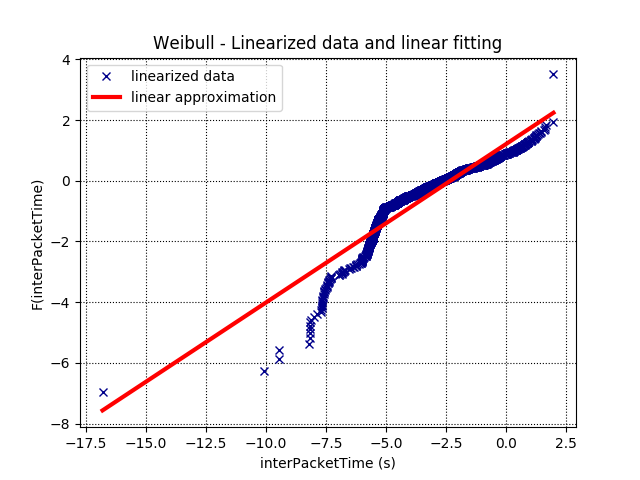
\includegraphics[height=50mm]{figures/apC/lr/Skype_Weibull_-_Linearized_data_and_linear_fitting}
  \label{fig:linearization}
}
%\hspace{0mm}
\subfloat[Cost function $J_\nabla$ of the linear regression]{
  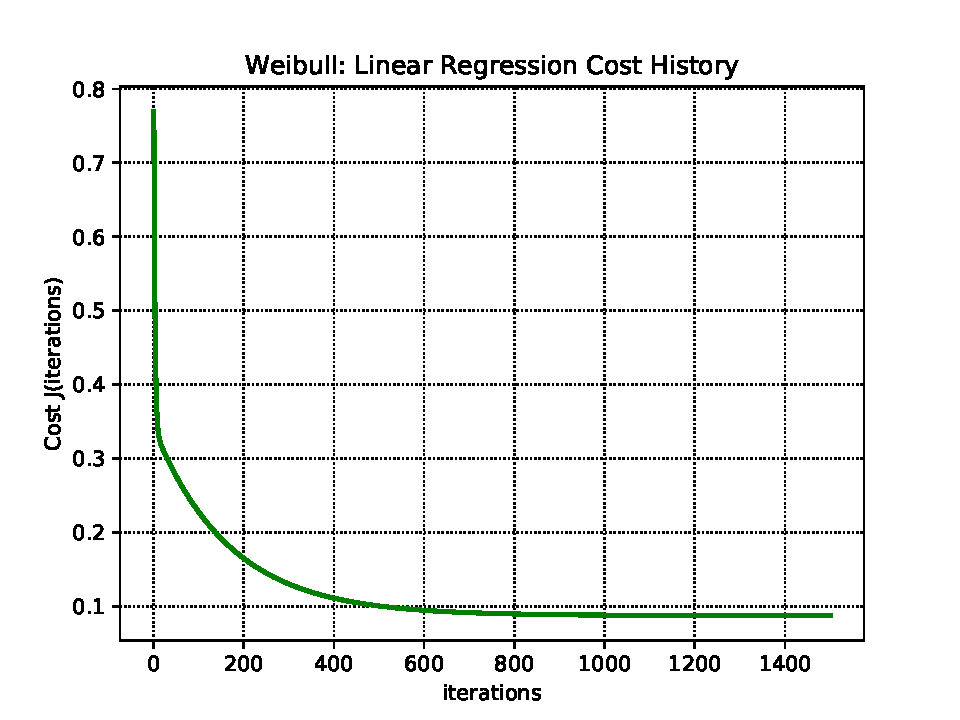
\includegraphics[height=50mm]{figures/apC/lr/Skype_Weibull_-_Cost_J(iterations)_convergence}
  \label{fig:cost}
}
\label{fig:linearization-cost}
\caption{Linearized data and cost function $J_\nabla$ of weibull linear regression}
\end{figure}


\subsubsection{Direct Estimation}

The expected value  $E(X)$ and variance $Var(X)$ of a random variable $X$ of some distributions are closely related to its parameters. Since the average $\bar{\mu}$ and its standard deviation$\bar{\sigma}$ are in general good approximations for the expected value and variance, we use them to estimate parameters.

Following the notation presented at table~\ref{tab:distributions-equations}, we have for the normal distribution the following ordered pair of parameters:

\begin{equation}
(\hat{\mu}, \hat{\sigma}) = (\bar{\mu}, \bar{\sigma})
\end{equation}

For the exponential distribution $E(X) = \frac{1}{\lambda}$. Therefore:

\begin{equation}
\hat{\lambda} = \frac{1}{\hat{\mu}}
\end{equation} 

\subsubsection{Maximum Likelihood}

The maximum likelihood estimation, is a method for estimation of The maximum likelihood estimation, is a method for estimation of The maximum likelihood estimation, is a method for estimation of parameters, winch maximizes the likelihood function. We explain in details this subject in Appendix~\ref{ap:revision-probability}. Using this method for the Pareto distribution;  it is possible to derive the following equations for its parameters: 


\begin{equation}
\hat{x_{m}} = \min_{i = 0, ..., m}\{x_{i}\}
\end{equation} 

\begin{equation}
\hat{\alpha} = \frac{n}{ \sum_{i = 0}^{m}(\ln{(x_{i}) - \ln(\hat{x_{m}})})  }
\end{equation} 

where $m$ is the sample(dataset) size.

\subsubsection{\textit{AIC} and \textit{BIC}}


Suppose that we have an statistical model $M$ of some dataset ${\boldsymbol{x} = \{x_1, ..., x_n}\}$, with $n$ independent and identically distributed observations of a random variable $X$. This model can be expressed by a PDF $f(x| \boldsymbol{\theta})$, where $\boldsymbol{\theta}$ a vector of parameter of the PDF, $\boldsymbol{\theta} \in \mathbb{R}^{k}$ ($k$ is the number of parameters). The  likelihood function  of this model $M$ is given by:

\begin{equation}
L(\boldsymbol{\theta}|\boldsymbol{x} ) =  f(x_1|\boldsymbol{\theta})\cdot...\cdot f(x_n|\boldsymbol{\theta}) = \prod_{i = 1}^{n}f(x_i|\boldsymbol{\theta})
\end{equation}

Now, suppose we are trying to estimate the best statistical model, from a set ${M_1, ..., M_n}$, each one whit an estimated vector of parameters  ${\boldsymbol{\hat{\theta_1}}}, ..., {\boldsymbol{\hat{\theta_n}}}$. $AIC$ and $BIC$ are defined by:

\begin{equation}
\label{eq:aic}
AIC = 2k - \ln(L(\boldsymbol{\hat{\theta}}|\boldsymbol{x}))
\end{equation}

\begin{equation}
\label{eq:bic}
BIC = k\ln(n) - \ln(L(\boldsymbol{\hat{\theta}}|\boldsymbol{x}))
\end{equation}

In both cases, the preferred model $M_i$, is the one with the smaller value of $AIC_i$ or $BIC_i$.


\subsection{Cross-validation method: Theoretical Foundation of the Cost Function}

To test if $AIC$ and $BIC$ do perform well, we had to answer two questions:

\begin{itemize}
\item[\#1] How do we evaluate if stochastic models and network traffic are playing well according to the expected?
\item[\#2] What reliable and trustable methods exist in the literature could we use to compare with $AIC$ and $BIC$?
\end{itemize}

To answer question \#1, the first thing is finding how well do a model can explain a given dataset. To answer this question  we find two widely adopted alternatives:

\begin{itemize}
\item \textbf{r-square}: applied just for linear regression, and measures how well a linearization can explain the data
\item \textbf{Pearson correlation coefficient}: can measures how well two random variables relate to each other.
\end{itemize}

Therefore, the metric that best satisfies our needs is the Pearson correlation coefficient.  The two random variables in question are the cross-validation dataset, and random values generated by the stochastic model.  We compared it repeatedly (30 times) to obtain a small enough confidence interval.  Its value goes from -1 to +1. +1 means a perfect direct linear correlation. "-1" indicates a perfect inverse linear correlation."0" means no linear correlation. So, as close the result reaches "1", more similar are the inter-packet times to the original values. To estimate it, we use the Octave’s function \texttt{corr()}. 


After addressing the question on the quality of data generated by the model, we need to evaluate the quality for actual, real network traffic, following the guidelines presented on chapter~\ref{ch:literature-review}, where we had defined four metric classes:

\begin{enumerate}
\item  Packet-level metrics
\item  Flow level metrics
\item  Scaling characteristics
\item  QoS/QoE related metrics
\end{enumerate}

Since we do not distinguish the traffic between flows, neither evaluate  QoS/QoE metrics, we could not directly extract metrics from these classes. Considering packet sizes in the first category is out of scope for our work and has been already studied in the literature.

On the metric class (1), the authors mention that the most common metric widely adopted is throughput. We can calculate the throughput on packets per second or byte rate. Both measures can be estimated using the mean inter-packet time.
The mean packet rate per second can be estimated by:

\begin{equation}
\label{eq:pps-mean}
packet throughput = 1 / (mean inter-packet time)
\end{equation}

So knowing the average packet size, we can estimate the byte by:

\begin{equation}
\label{eq:th-mean}
byte throughput = (average packet size)/(mean inter-packet time)
\end{equation}

Therefore a good approximation on the average inter-packet time means a reasonable estimate on the traffic throughout as well. Another metric cited by the authors in the scope is the analysis of inter-packet size distributions. Researchers typically make distribution analyzes via graphical interpretation. Seeing its importance, we show as an example one of our results on that matter, now on figure XX. This figure shows the comparison of four  CDF functions estimations for the \textit{lan-firewall-pcap}, with the cross-validation data. Works such as \cite{ditg-paper} \cite{sourcesonoff-paper}\cite{do-you-trust}\cite{harpoon-validation}\cite{moongen-paper}\cite{modelling-of-self-similar} did the same task, for their own purposes using the PDF or CDF distributions. We opted to present the CDF plot because we found it easier for discussion. However, since the goal of our work is to compare $AIC$ and $BIC$  with other possible rankings inspired in the literature, we had to abstract these plots in a single metric that represents the fitting quality. To this end, we use the (already mentioned)  Pearson correlation coefficient.

Finally, there is (3) Scaling characteristics, a well-known aspect of traffic modeling. From the seminal work of Leland et al. \cite{selfsimilar-ethernet}, we know that the ethernet traffic has a self-similar and fractal-like behavior. Some of the most important are the estimation of the Hurst exponent (used on the last mentioned paper) \cite{selfsimilar-ethernet}\cite{multi-player-online-game-self-similarity}\cite{wavelet-analysis-long-range}, Wavelet multiresolution analysis \cite{multi-player-online-game-self-similarity}\cite{wavelet-analysis-long-range}\cite{swing-paper}, power-law and power spectrum analysis, as suggested by \cite{modelling-of-self-similar}. However, to the best of our knowledge, there is no other method widespread as Hurst exponent and Wavelet analysis. The problem of wavelet for our purposes is that its interpretation is inherently graphical, and can be used to identify periodicities, white-noise, and self-similar characteristics on a long-range analysis, depending on the graphical behavior. However, for automatic model ranking, this approach is not practical.


On the other hand, the Hurst exponent ideal for this task, since it is a single value, and is a representation of the fractal dimension of the dataset.  Therefore, we choose to rank the scaling characteristics of our models, based on how close they can get from the estimation of the Hurst exponent of the cross-validation. We repeated the estimation for both cross-validation and synthetic dataset 30 times until we got a fair and small error margin. We did not consider in our analysis of other stochastic metrics,  such as the standard deviation of the dataset. Although the standard deviation is useful on the understanding of the nature of the traffic, we judge that it be redundant with the Hurst exponent estimation, since it is already a measure of the data variability. To determine this value, we use the function \texttt{hurst()} from Octave, which uses the rescaled range method. 

Therefore, we got three different rankings based on the literature, each of them giving their estimation of what model performs better. To do not prioritize any of these metrics, and provide a ponderated best result we created the so-called cost function $J$, which is an aggregator of results. Being $Cr$ the vector of correlations ordered from higher to the smaller, let $Me$ and $Hr$ defined by the absolute difference between average and hurt exponent of the estimated values and the original data-set, both ordered from the small to the high values. Letting $\phi(V, M)$ be an operator which gives the position of a model $M$ in a vector $V$, we define the cost function $J$ as:

\begin{equation}
\label{eq:cost-function}
J_M(M) = \phi(Cr, M) + \phi(Me, M) + \phi(Hr, M)
\end{equation}

The smaller is the cost $J_M$; the best is the model. For example, suppose a model m1 that has the best performance on the average inter-packet time estimation, but delivers smaller performance on data correlation and the Hurst exponent. That means, this model was able to overfit the mean inter-packet time representation but does a poor data representation on all the other cases. Since we are comparing seven models, this model can deliver the following cost estimation (counting starts from position 0):

\begin{equation}
\label{eq:cost-function-ex1}
J_M(M) = \phi(Cr, m_1) + \phi(Me, m_1) + \phi(Hr, m_1) = 6 + 0 + 6 = 12
\end{equation}

On the other hand, suppose a model m2 that performs as second best on all the tests. This one will have:

\begin{equation}
\label{eq:cost-function-ex2}
J_M(M) = \phi(Cr, m_2) + \phi(Me, m_2) + \phi(Hr, m_2) = 1 + 1 + 1 = 3
\end{equation}

Although model $m_1$, if used for traffic generation would perform well on the throughput representation, it is not fair that it goes ahead of the second model $m_2$, which performed pretty well on all the metrics. Therefore, we can safely say that  $m_2$ a better representation of inter-packet times, according to metrics typically adopted in the literature of network traffic and stochastic analysis. 


%%%%%%%%%%%%%%%%%%%%%%%%%%%%%%%%%%%%%%%%%%%%%%%%%%%%%%%%%%%%%%%%%%%%%%%%%%%%%%%
\subsection{Results}


%%%%%%%%%%%%%%%%%%%%%%%
% Simulation table
%%%%%%%%%%%%%%%%%%%%%%%
\begin{sidewaystable}[!htp]
\caption{Experimental results, including the estimated parameters and the BIC and AIC values of the four pcap traces.}
\scalebox{0.90}{ 
\centering
\begin{threeparttable}[t]
\begin{tabular}{lcccccccc}
\hline
\multicolumn{9}{c}{Trace}                                                                                                                                                 \\ \cline{2-9} 
Function        & AIC         &           & \multicolumn{2}{c}{Parameters}                           & AIC       & BIC       & \multicolumn{2}{c}{Parameters}                     \\ \hline
\multicolumn{5}{c}{skype-pcap}                                                                       & \multicolumn{4}{c}{lan-firewall-pcap}                                      \\ \hline
Cauchy          & $6.94E+03$  & $6.95E+03$  & $\gamma : 1.71E-04$     & $x_0 : 1.88E-01$     & $-2.29E+05$ & $-2.29E+05$ & $\gamma : 1.93E-02$     & $x_0 : -4.97E-02$    \\
Exponential(LR) & $-4.70E+01$ & $-4.28E+01$ & \multicolumn{2}{c}{$\lambda : 1.79E+00$}              & $-2.22E+06$ & $-2.22E+06$ & \multicolumn{2}{c}{$\lambda : 4.05E-01$}            \\
Exponential(Me) & $-2.16E+02$ & $-2.12E+02$ & \multicolumn{2}{c}{$\lambda : 3.45E+00$}          & $3.63E+05$  & $3.63E+05$  & \multicolumn{2}{c}{$\lambda : 1.13E+02$}        \\
Normal          & $1.21E+03$  & $1.22E+03$  & $\mu : 2.90E-01$      & $\sigma : 6.95E-01$    & $-1.48E+06$ & $-1.48E+06$ & $\mu : 8.85E-03$      & $\sigma : 3.49E-02$    \\
Pareto(LR)      & $3.38E+03$  & $3.39E+03$  & $\alpha : 4.28E-01$     & $x_m :  5.00E-08$     & $Inf \tnote{1}$       & $Inf \tnote{1}$       & $\alpha : 2.51E-01$     & $x_m :  5.00E-08$     \\
Pareto(MLH)     & $1.88E+02$  & $1.97E+02$  & $\alpha : 7.48E-02$ & $x_m :  5.00E-08$ & $-1.80E+06$ & $-1.80E+06$ & $\alpha : 1.15E-01$ & $x_m :  5.00E-08$ \\
Weibull         & $-1.15E+03$ & $-1.14E+03$ &                             & $\beta : 9.68E-02$ & $-1.97E+06$ & $-1.97E+06$ & $\alpha : 3.46E-01$    & $\beta : 1.79E-03$ \\ \hline
\multicolumn{5}{c}{lan-gateway-pcap}                                                                 & \multicolumn{4}{c}{wan-pcap}                                               \\ \hline
Cauchy          & $3.65E+06$  & $3.65E+06$  & $\gamma : 1.95$         & $x_0 : -4.45E+03$    & $2.99E+07$  & $2.99E+07$  & $\gamma : 8.17E+02$     & $x_0 : -4.45E+03$    \\
Exponential(LR) & $3.67E+06$  & $3.67E+06$  & \multicolumn{2}{c}{$\lambda : 9.75E-03$}              & $2.84E+07$  & $2.84E+07$  & \multicolumn{2}{c}{$\lambda : 2.20E-05$}            \\
Exponential(Me) & $-5.44E+06$ & $-5.44E+06$ & \multicolumn{2}{c}{$\lambda : 2.64E+03$}          & $-3.29E+07$ & $-3.29E+07$ & \multicolumn{2}{c}{$\lambda : 6.58E+05$}        \\
Normal          & $-4.67E+06$ & $-4.67E+06$ & $\mu : 3.79E-04$      & $\sigma : 1.00E-06$    & $-3.19E+07$ & $-3.19E+07$ & $\mu : 2.00E-06$      & $\sigma : 1.00E-06$    \\
Pareto(LR)      & $-5.13E+06$ & $-5.13E+06$ & $\alpha : 1.49E-01$     & $x_m :  5.00E-08$     & $4.51E+07$  & $4.51E+07$  & $\alpha :  4.00E-14 \tnote{2}$     & $x_m :  5.00E-08$     \\
Pareto(MLH)     & $-5.13E+06$ & $-5.13E+06$ & $\alpha : 1.36E-01$ & $x_m :  5.00E-08$ & $-3.13E+07$ & $-3.13E+07$ & $\alpha : 3.39E-01$ & $x_m : 5.00E-08$ \\
Weibull         & $-5.50E+06$ & $-5.50E+06$ & $\alpha : 2.81E-01$    & $\beta : 1.00E-06$ & $-2.73E+07$ & $-2.73E+07$ & $\alpha : 7.64E-02$    & $\beta : 1.00E-06$ \\ \hline
\end{tabular}
            \begin{tablenotes}
            \item[1] The computation of the likelihood function has exceeded the computational precision used, so it was the highest AIC and BIC  for this trace.
            \item[2] The linear regression did not converge to a valid value, so we used a small value instead to perform the computations.
            \end{tablenotes}
\end{threeparttable}
}
\label{tab:prototype-results}
\end{sidewaystable}


%%%%%%%%%%%%%%%%%%%%%%%
% Logscale Skype
%%%%%%%%%%%%%%%%%%%%%%%
\begin{figure}[pht!]
\centering
\subfloat[Chauchy]{
  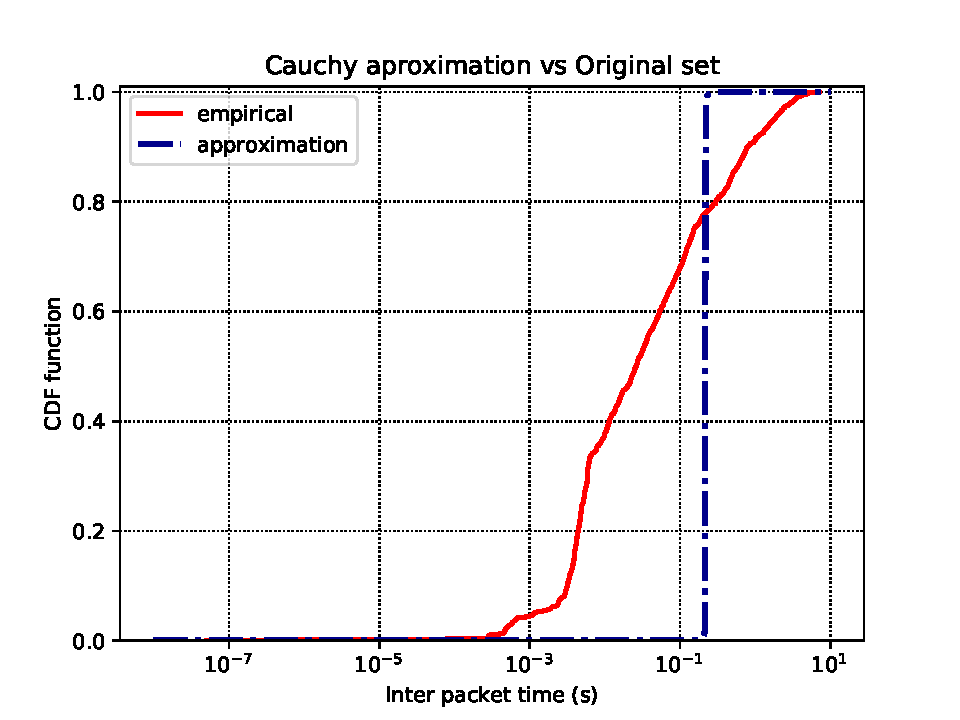
\includegraphics[width=62mm]{figures/ch4/Skype_Log_-_Cauchy_aproximation_vs_Original_set}
}
\subfloat[Exponential(LR)]{
  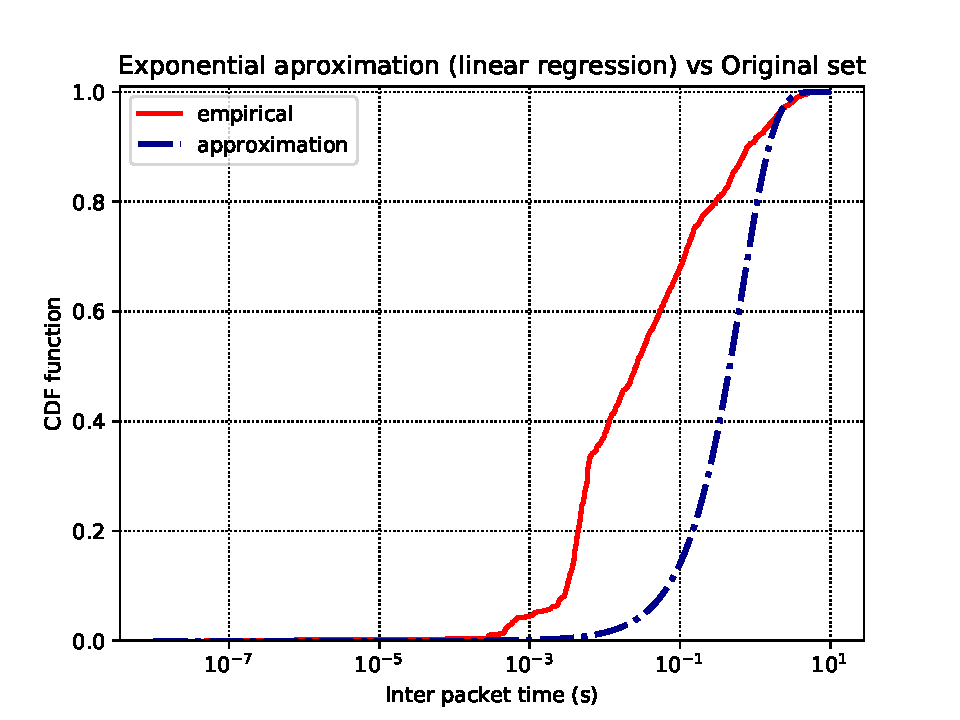
\includegraphics[width=62mm]{figures/ch4/Skype_Log_-_Exponential_aproximation_(linear_regression)_vs_Original_set}
}
\hspace{0mm}
\subfloat[Exponential(Me)]{
  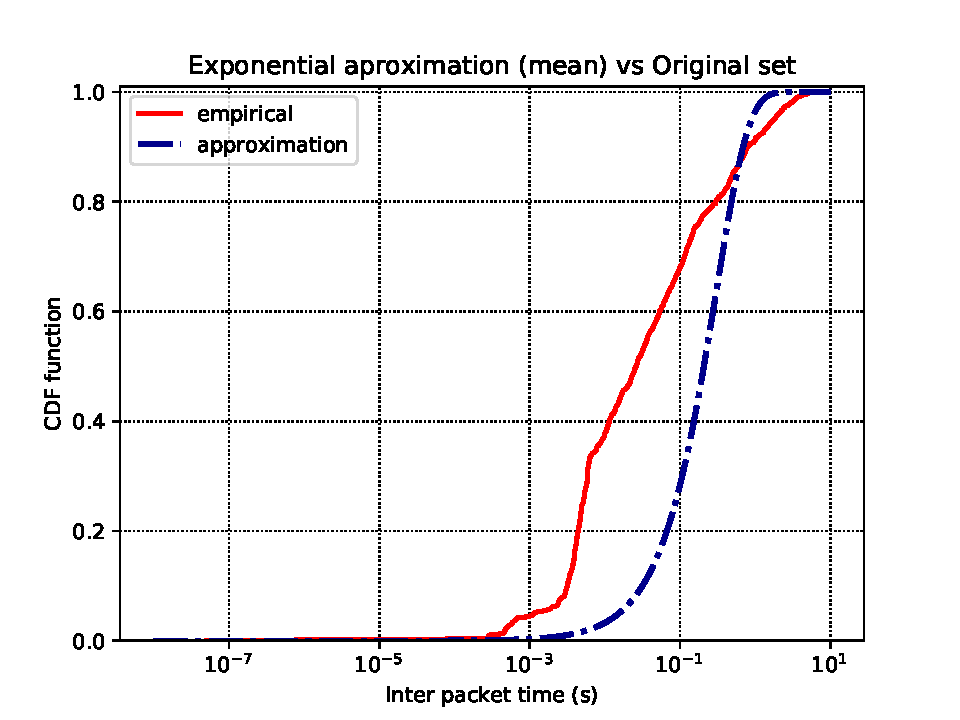
\includegraphics[width=62mm]{figures/ch4/Skype_Log_-_Exponential_aproximation_(mean)_vs_Original_set}
}
\subfloat[Normal]{
  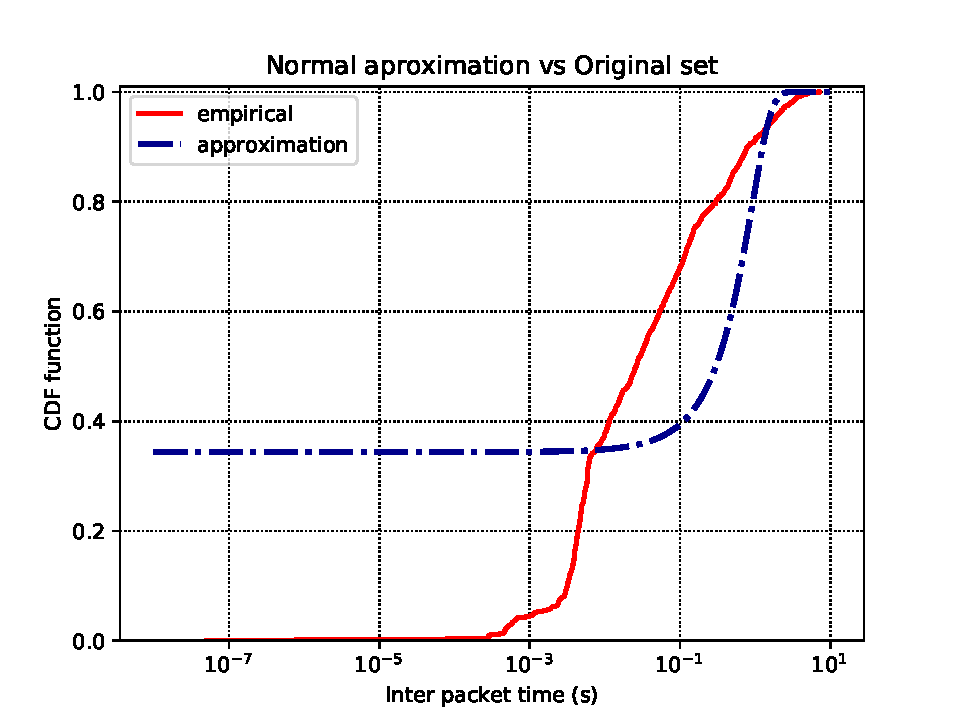
\includegraphics[width=62mm]{figures/ch4/Skype_Log_-_Normal_aproximation_vs_Original_set}
}
\hspace{0mm}
\subfloat[Pareto(LR)]{
  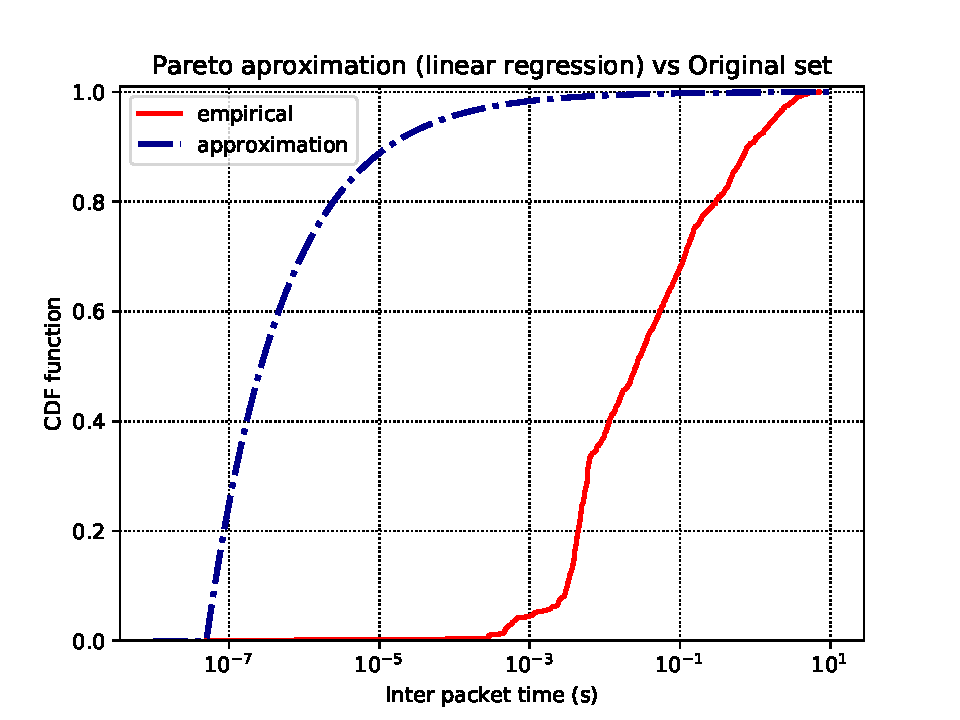
\includegraphics[width=62mm]{figures/ch4/Skype_Log_-_Pareto_aproximation_(linear_regression)_vs_Original_set}
}
\subfloat[Pareto(MLH)]{
  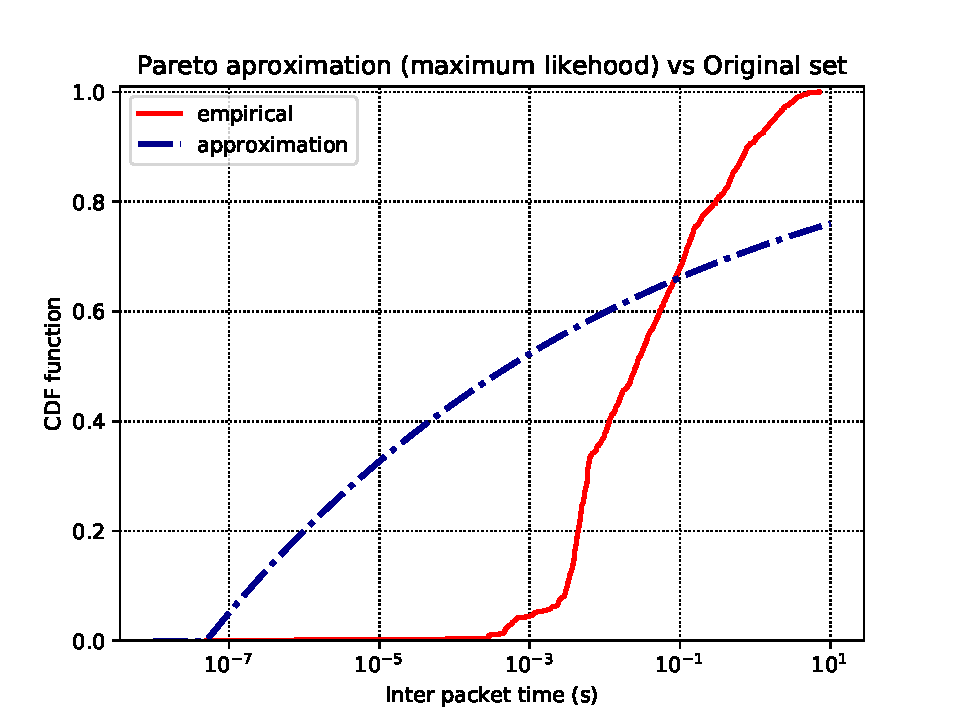
\includegraphics[width=62mm]{figures/ch4/Skype_Log_-_Pareto_aproximation_(maximum_likehood)_vs_Original_set}
}
\hspace{0mm}
\subfloat[Weibull]{
  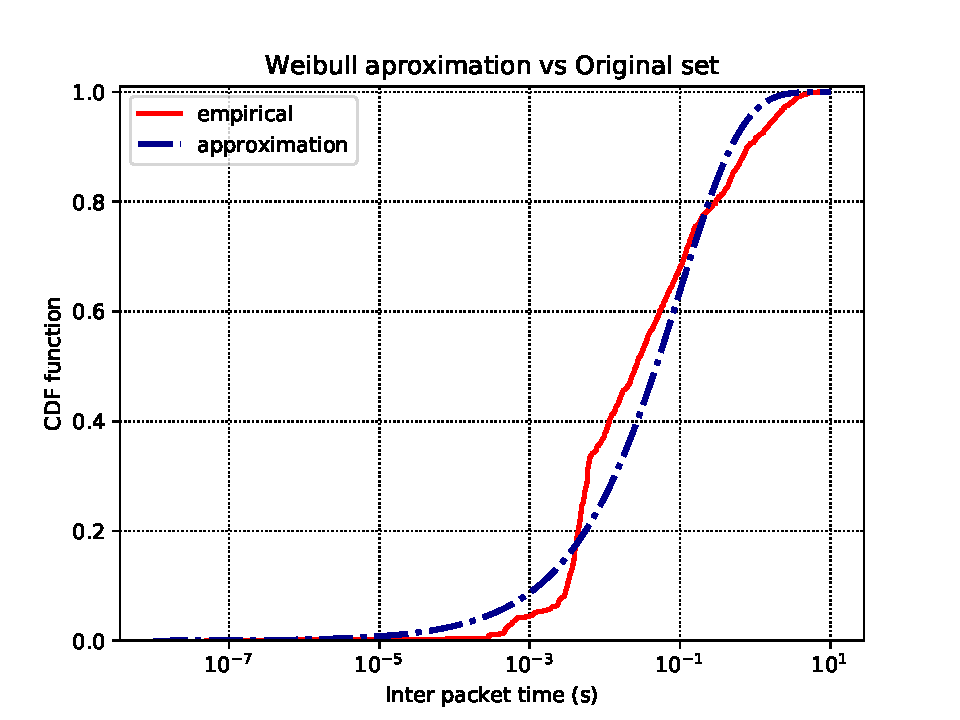
\includegraphics[width=62mm]{figures/ch4/Skype_Log_-_Weibull_aproximation_vs_Original_set}
}
\caption{CDF functions for the approximations of \textit{skype-pcap} inter  packet times, of many stochastic functions.}
\label{fig:aproximation-original-cdf}
\end{figure}


%%%%%%%%%%%%%%%%%%%%%%%
% QQplots Skype
%%%%%%%%%%%%%%%%%%%%%%%
\begin{figure}[pht!]
    \centering
    \subfloat[Chauchy]{
        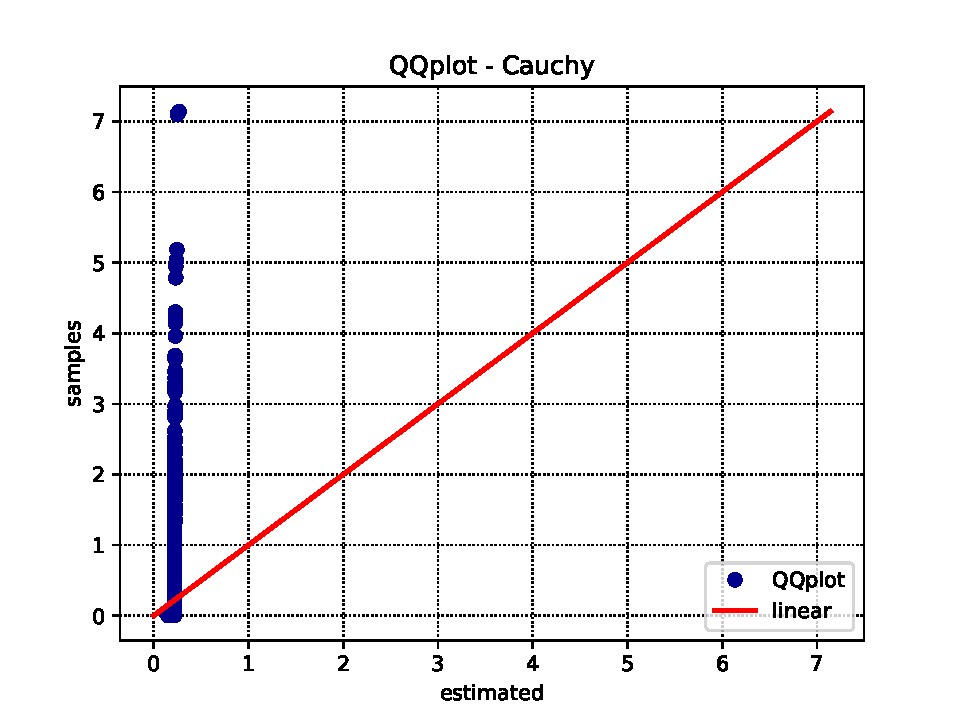
\includegraphics[width=62mm]{figures/ch4/Skype_QQplot_-_Cauchy}
    }
    \subfloat[Exponential(LR)]{
        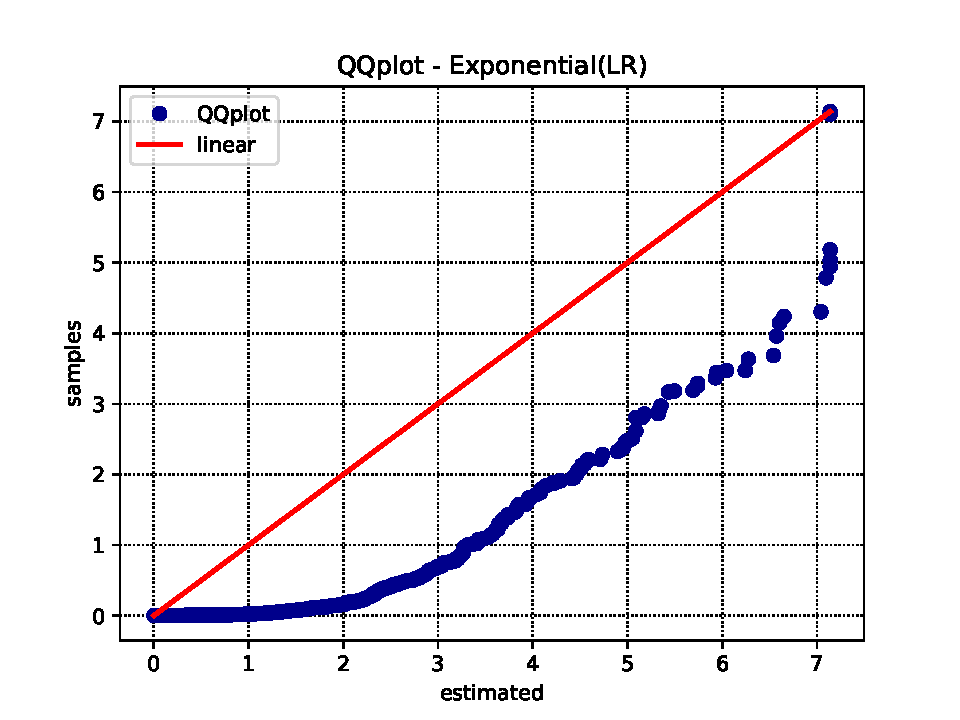
\includegraphics[width=62mm]{figures/ch4/Skype_QQplot_-_Exponential(LR)}
    }
    \hspace{0mm}
    \subfloat[Exponential(Me)]{
        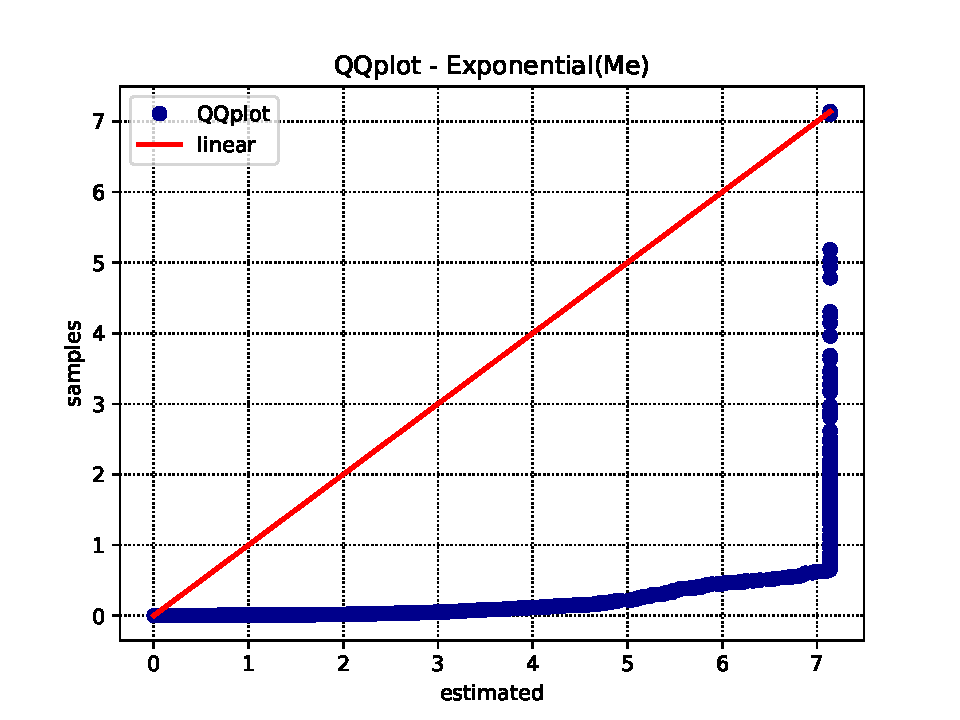
\includegraphics[width=62mm]{figures/ch4/Skype_QQplot_-_Exponential(Me)}
    }
    \subfloat[Normal]{
        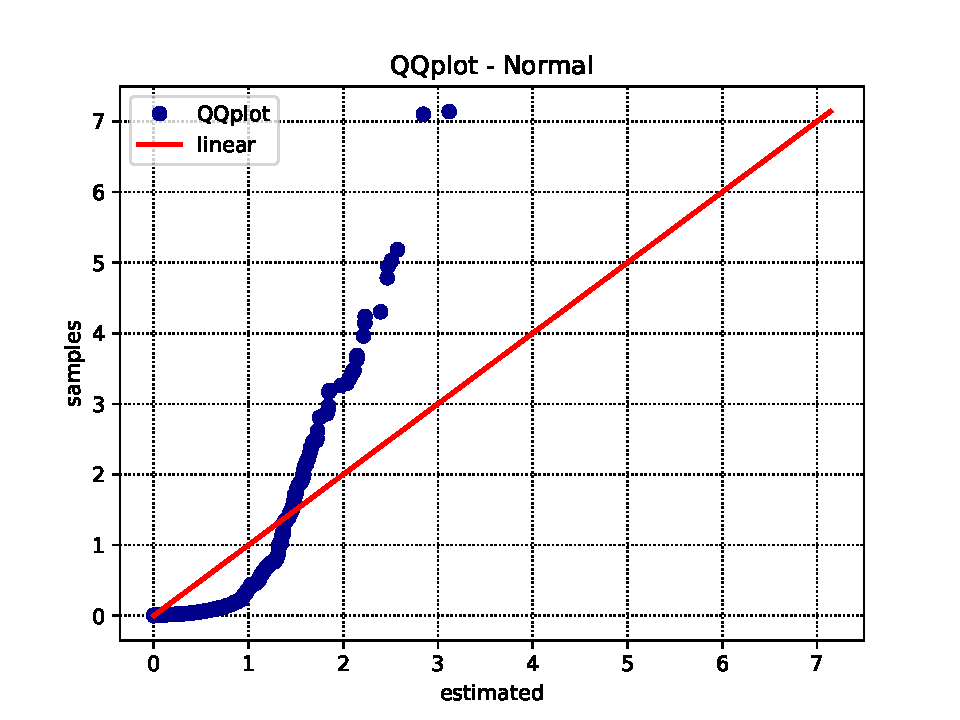
\includegraphics[width=62mm]{figures/ch4/Skype_QQplot_-_Normal}
    }
    \hspace{0mm}
    \subfloat[Pareto(LR)]{
        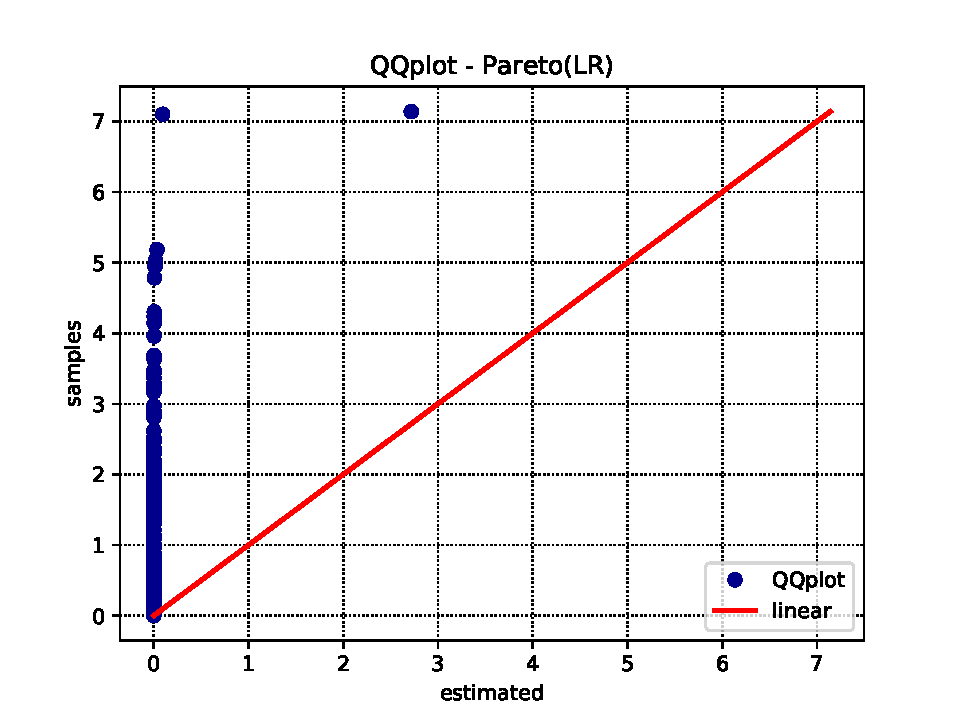
\includegraphics[width=62mm]{figures/ch4/Skype_QQplot_-_Pareto(LR)}
    }
    \subfloat[Pareto(MLH)]{
        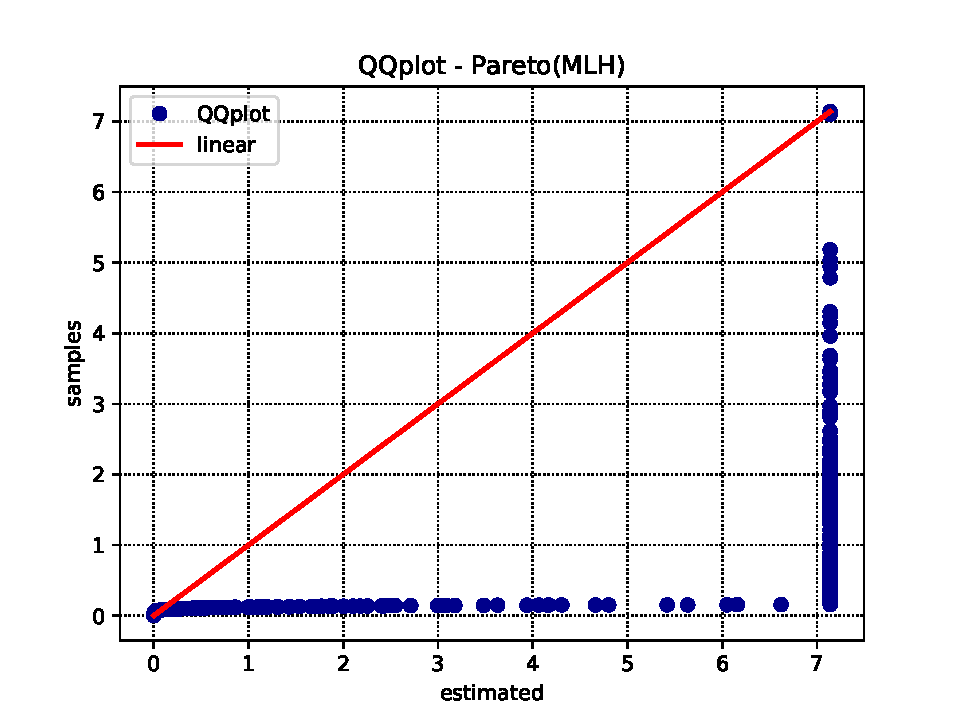
\includegraphics[width=62mm]{figures/ch4/Skype_QQplot_-_Pareto(MLH)}
    }
    \hspace{0mm}
    \subfloat[Weibull]{
        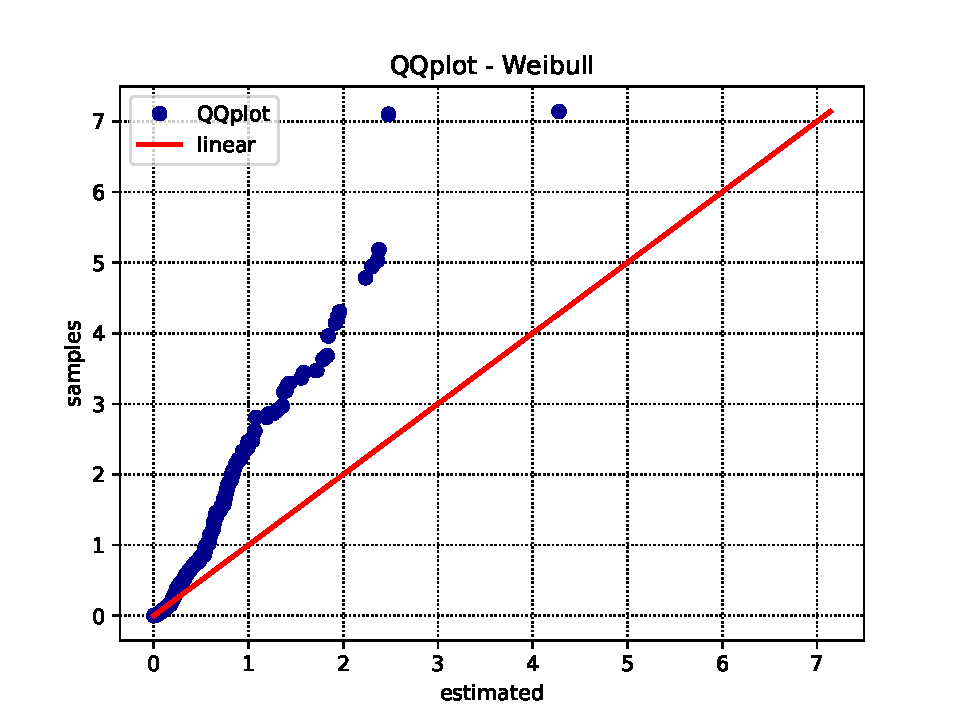
\includegraphics[width=62mm]{figures/ch4/Skype_QQplot_-_Weibull}
    }
    \caption{CDF functions for the approximations of \textit{skype-pcap} inter packet times, of many stochastic functions.}
    \label{fig:qq-skype}
\end{figure}


\begin{figure}[ph]
\centering
%%%%%%%%%%%%%%%%%%%%%%%
% Skype  - Correlation, Hurst, Mean Standard Deviation
%%%%%%%%%%%%%%%%%%%%%%%
\begin{figure}[H]
    \centering
    \subfloat[Correlation]{
        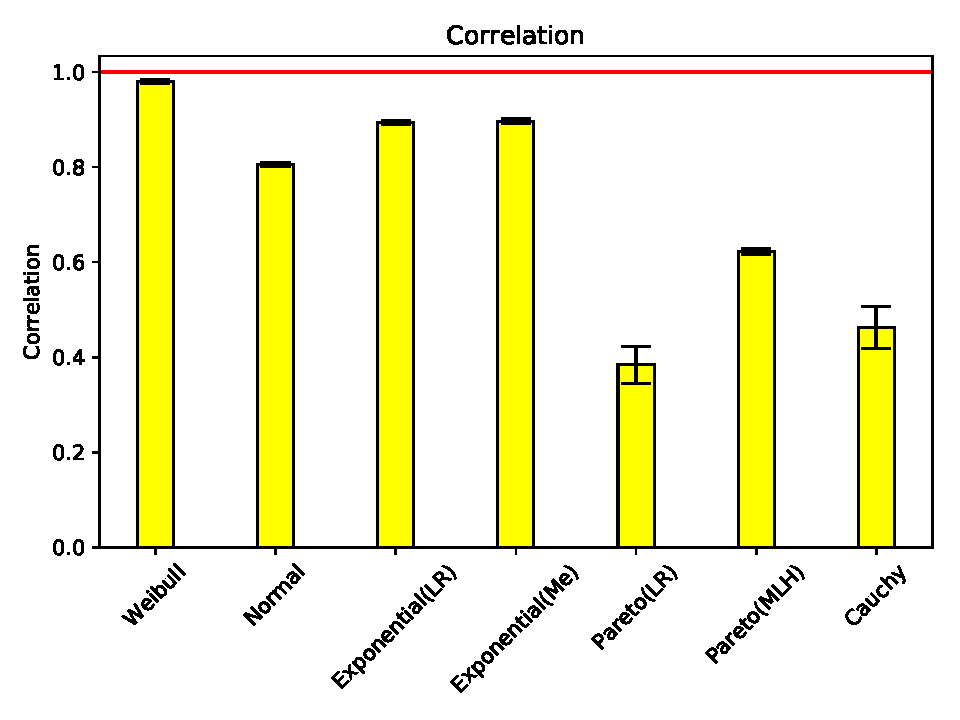
\includegraphics[width=60mm]{figures/ch4/Skype_Correlation}
        \label{correlation-skype}
    }
    \hspace{0mm}
    \subfloat[Hust Exponent]{
        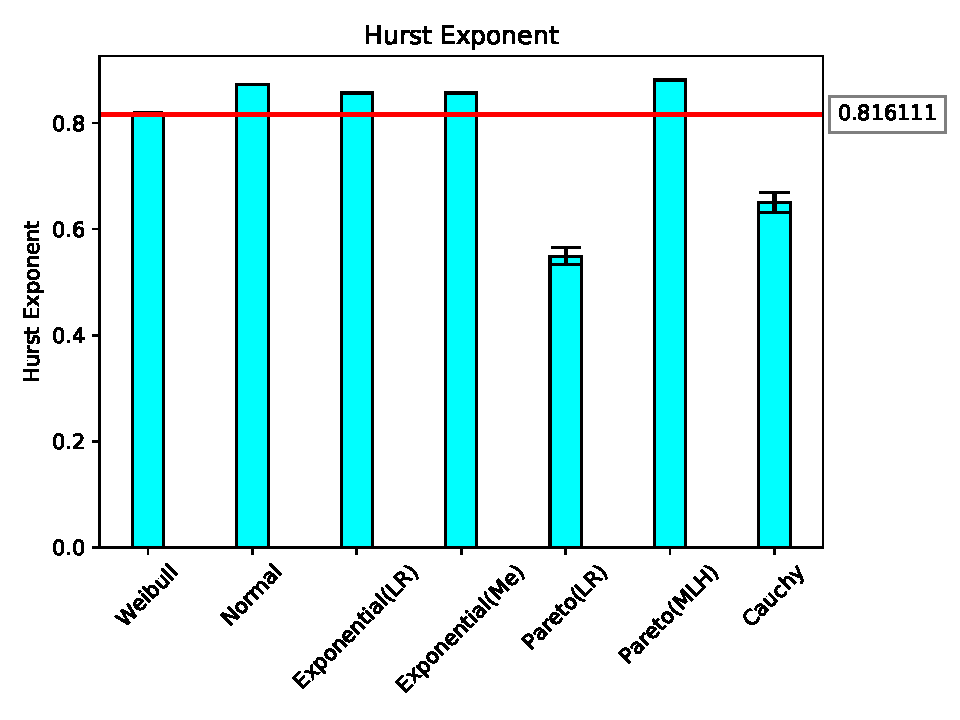
\includegraphics[width=60mm]{figures/ch4/Skype_Hurst_Exponent}
        \label{hurst-skype}
    }
    \hspace{0mm}
    \subfloat[Mean]{
        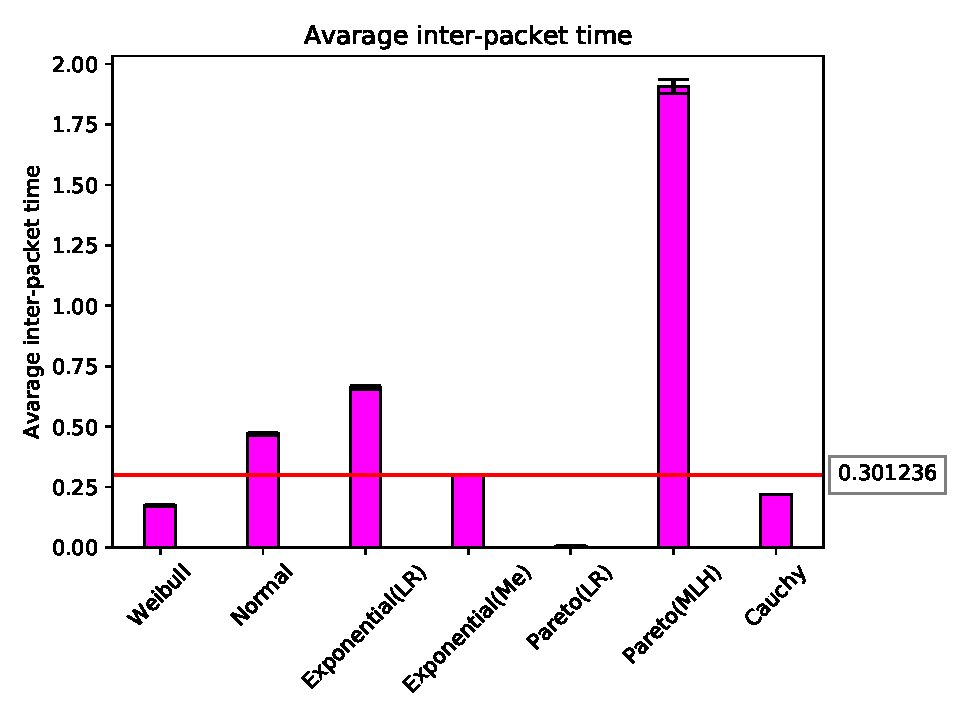
\includegraphics[width=60mm]{figures/ch4/Skype_Mean}
        \label{mean-skype}
    }
    \hspace{0mm}
    \subfloat[Standard Deviation]{
        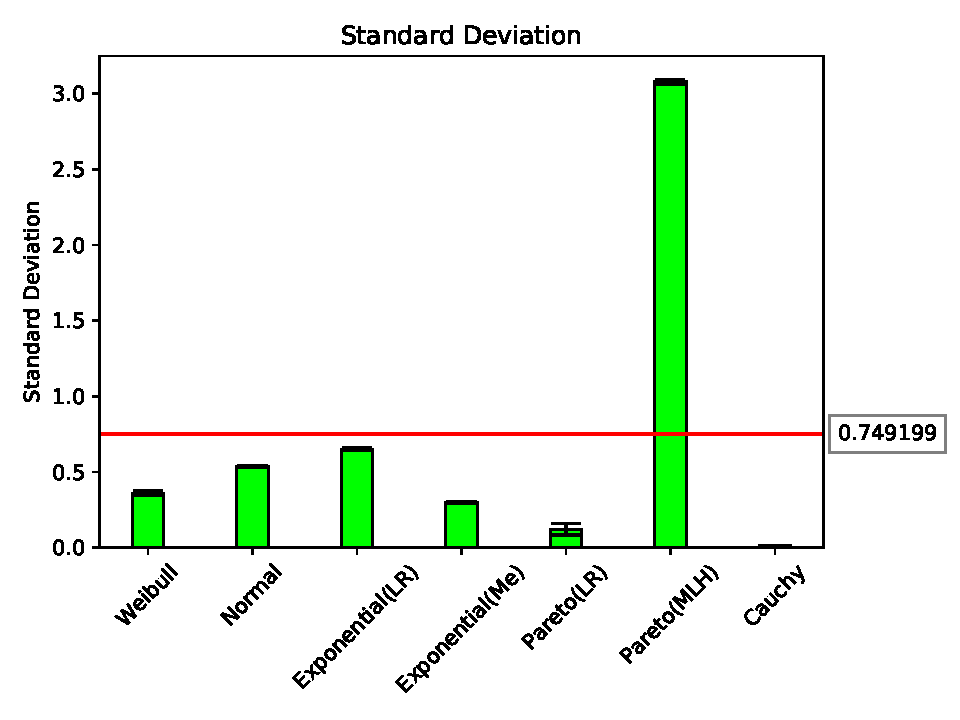
\includegraphics[width=60mm]{figures/ch4/Skype_Standard_Deviation}
        \label{std-skype}
    }
    \caption{Statistical parameters of \textit{skype-pcap} and its approximations}
    \label{fig:correlation-hurst-skype-pcap}
\end{figure}
%%%%%%%%%%%%%%%%%%%%%%%
% lan-gateway -  Correlation, Hurst, Mean Standard Deviation
%%%%%%%%%%%%%%%%%%%%%%%
\begin{figure}[H]
    \centering
    \subfloat[Correlation]{
        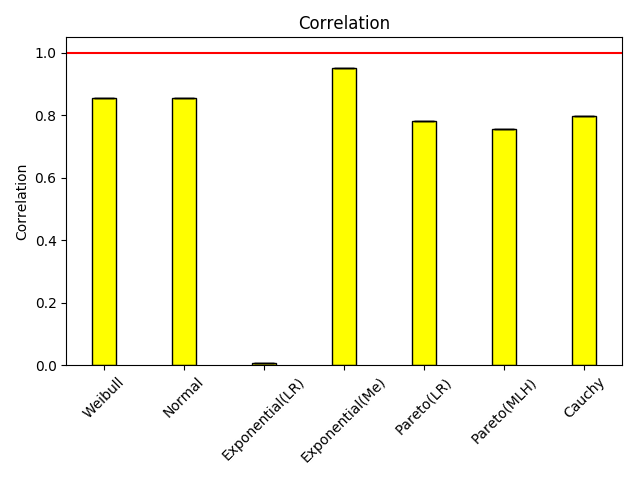
\includegraphics[width=60mm]{figures/ch4/bigFlows_Correlation}
        \label{lan-gateway-correlation-skype}
    }
    \hspace{0mm}
    \subfloat[Hust Exponent]{
        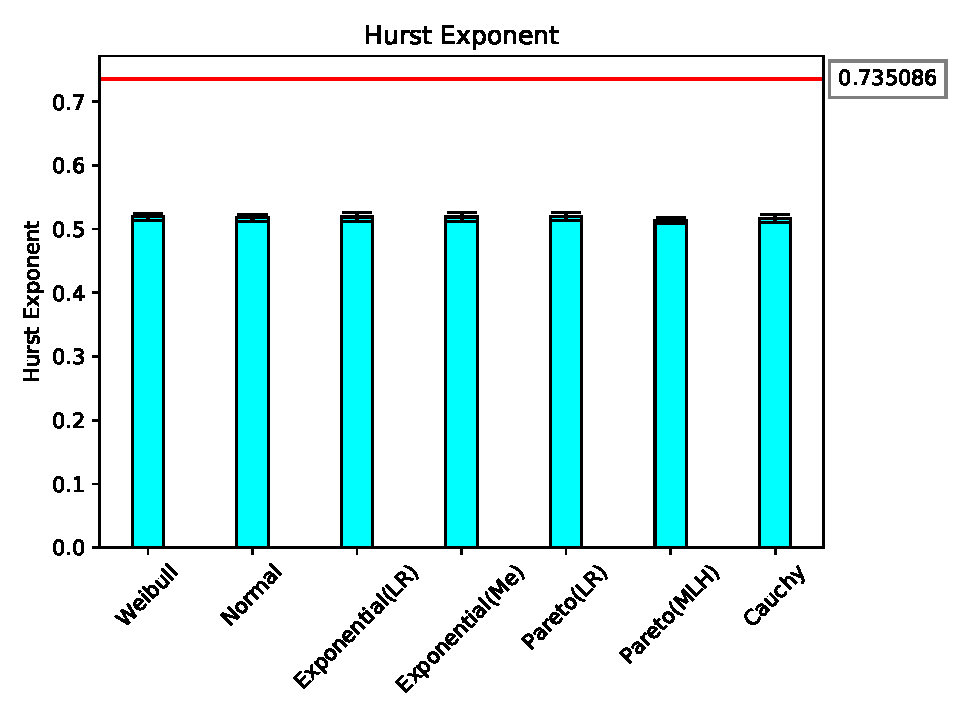
\includegraphics[width=60mm]{figures/ch4/bigFlows_Hurst_Exponent}
        \label{lan-gateway-hurst-skype}
    }
    \hspace{0mm}
    \subfloat[Mean]{
        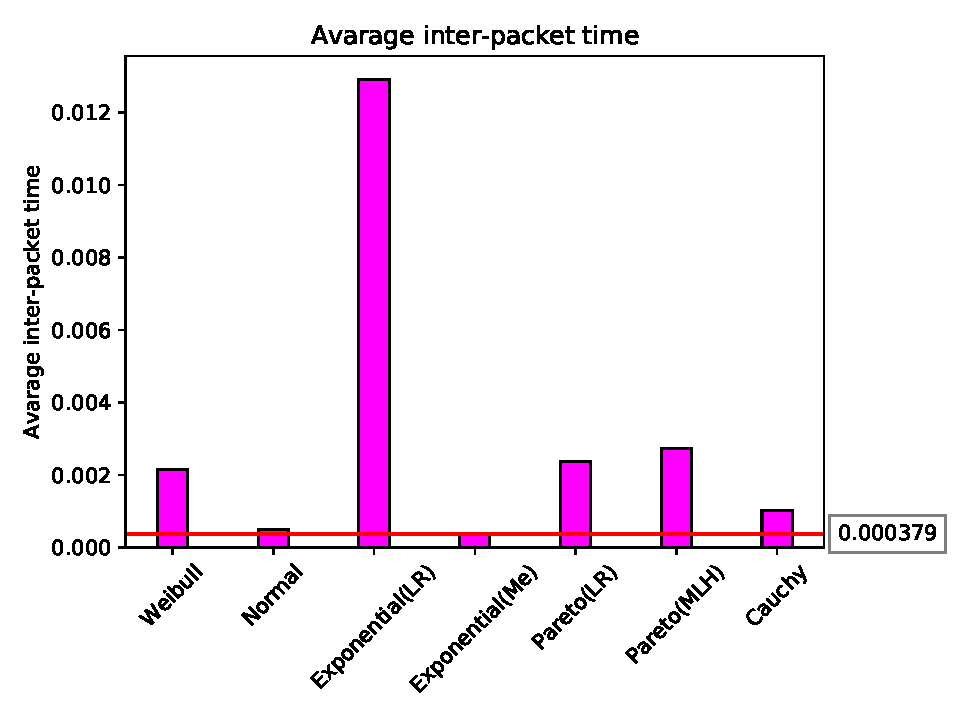
\includegraphics[width=60mm]{figures/ch4/bigFlows_Mean}
        \label{lan-gateway-mean-skype}
    }
    \hspace{0mm}
    \subfloat[Standard Deviation]{
        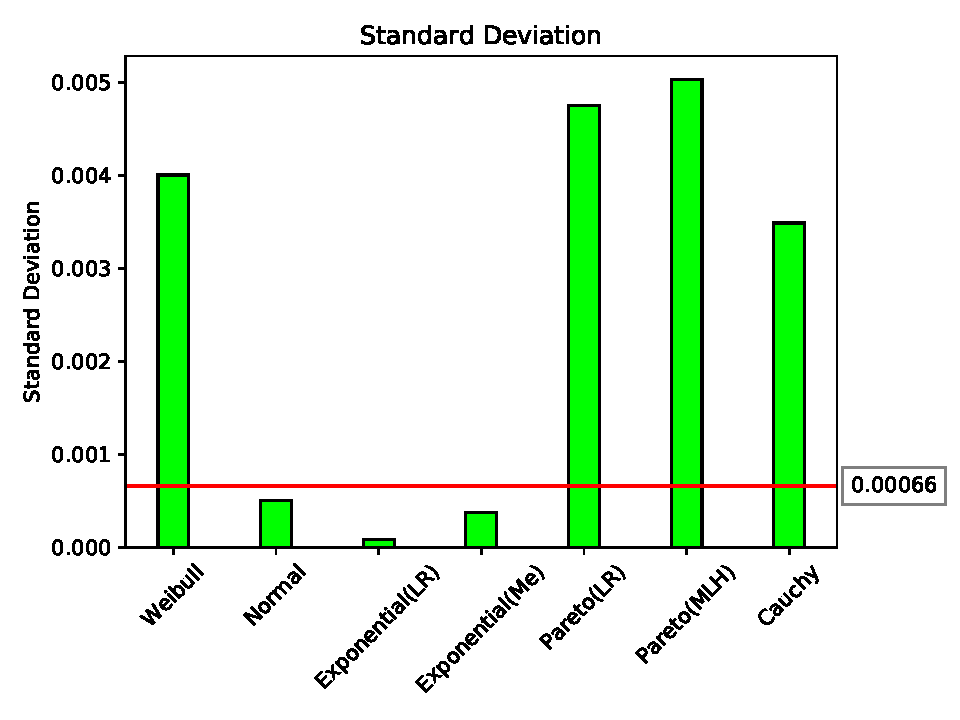
\includegraphics[width=60mm]{figures/ch4/bigFlows_Standard_Deviation}
        \label{lan-gateway-std-skype}
    }
    \caption{Statistical parameters of \textit{lan-gateway-pcap} and its approximations}
    \label{fig:correlation-hurst-lan-gateway-pcap}
\end{figure}
\end{figure}

\begin{figure}[ph]
%%%%%%%%%%%%%%%%%%%%%%%
% lanDirunal  - correlation, Hurst, Mean Standard Deviation
%%%%%%%%%%%%%%%%%%%%%%%
\begin{figure}[H]
    \centering
    \subfloat[Correlation]{
        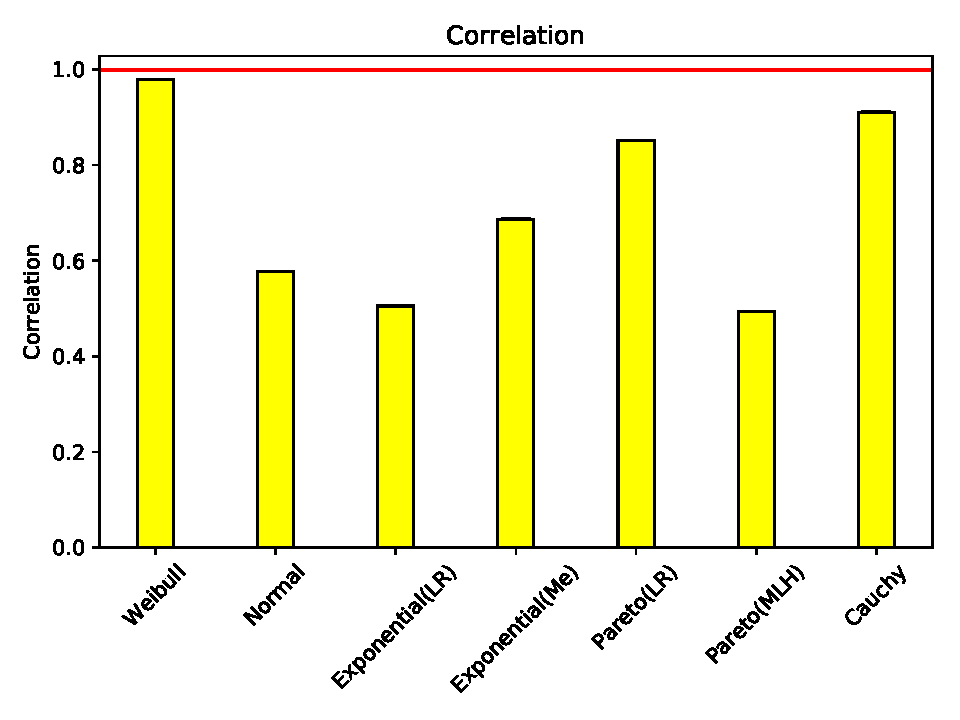
\includegraphics[width=60mm]{figures/ch4/Lan_Correlation}
        \label{Lan-correlation-skype}
    }
    \hspace{0mm}
    \subfloat[Hust Exponent]{
        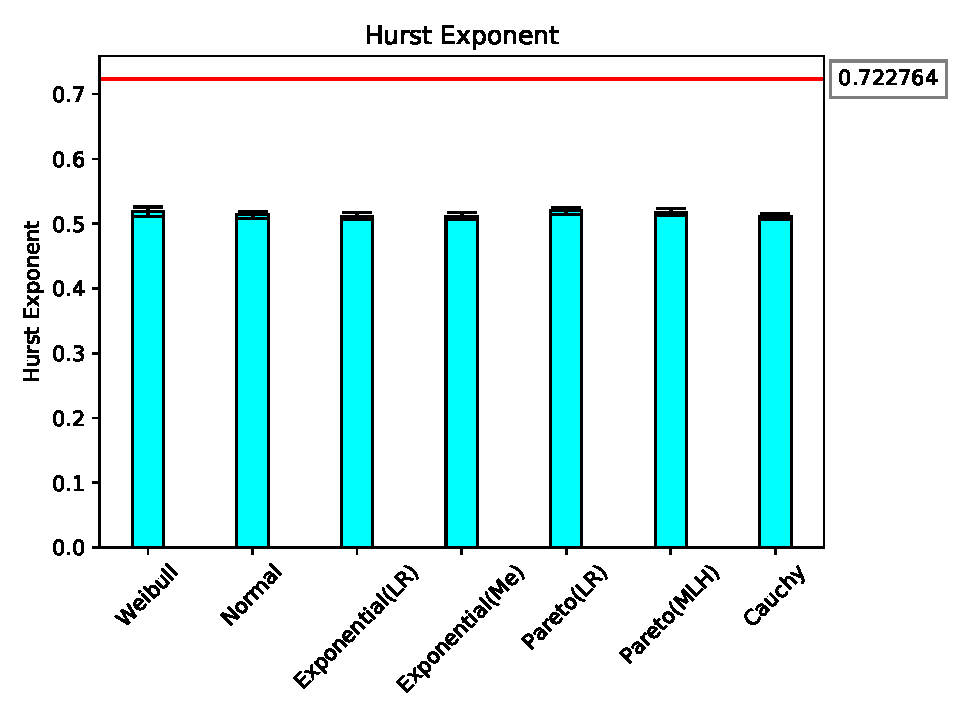
\includegraphics[width=60mm]{figures/ch4/Lan_Hurst_Exponent}
        \label{Lan-hurst-skype}
    }
    \hspace{0mm}
    \subfloat[Mean]{
        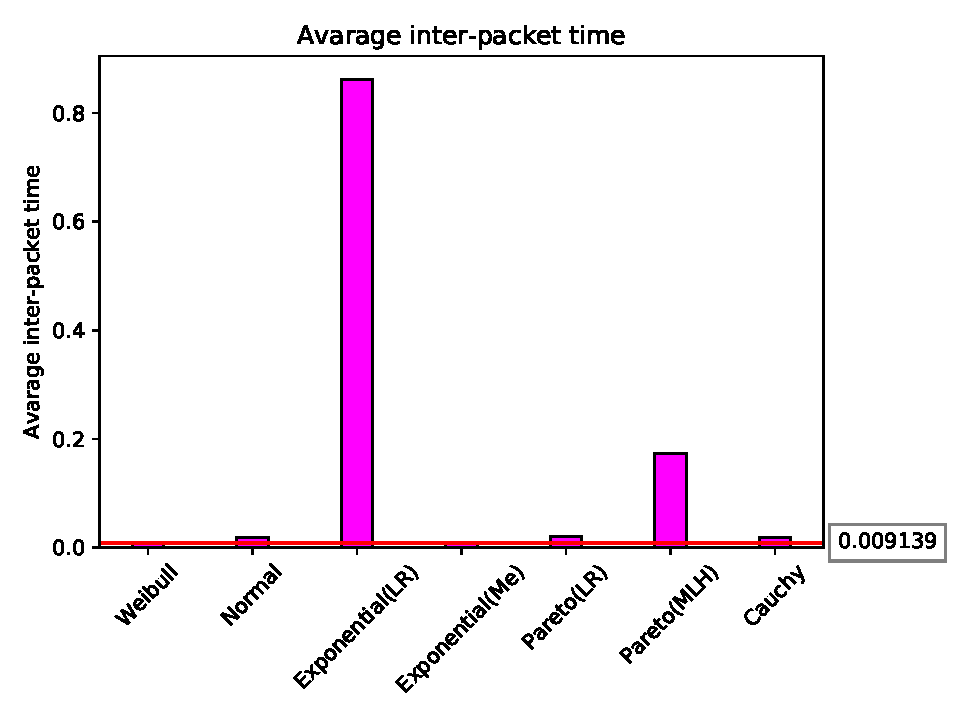
\includegraphics[width=60mm]{figures/ch4/Lan_Mean}
        \label{Lan-mean-skype}
    }
    \hspace{0mm}
    \subfloat[Standard Deviation]{
        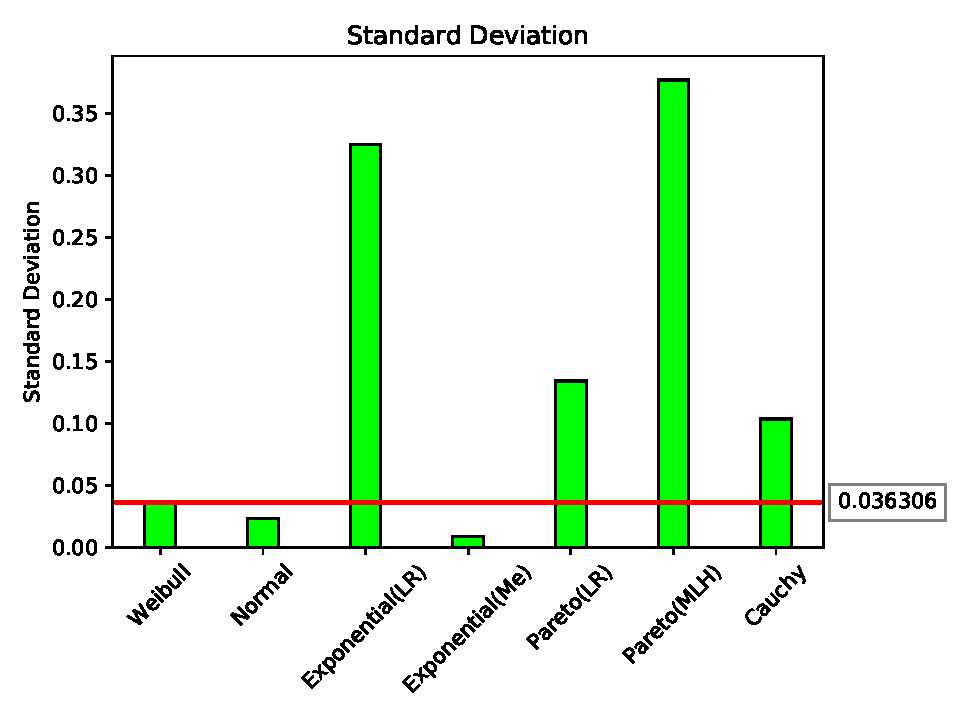
\includegraphics[width=60mm]{figures/ch4/Lan_Standard_Deviation}
        \label{Lan-std-skype}
    }
    \caption{Statistical parameters of \textit{lan-firewall-pcap} and its approximations}
    \label{fig:correlation-hurst-Lan-pcap}
\end{figure}
%%%%%%%%%%%%%%%%%%%%%%%
% Wan - correlation, Hurst, Mean Standard Deviation
%%%%%%%%%%%%%%%%%%%%%%%
\begin{figure}[H]
    \centering
    \subfloat[Correlation]{
        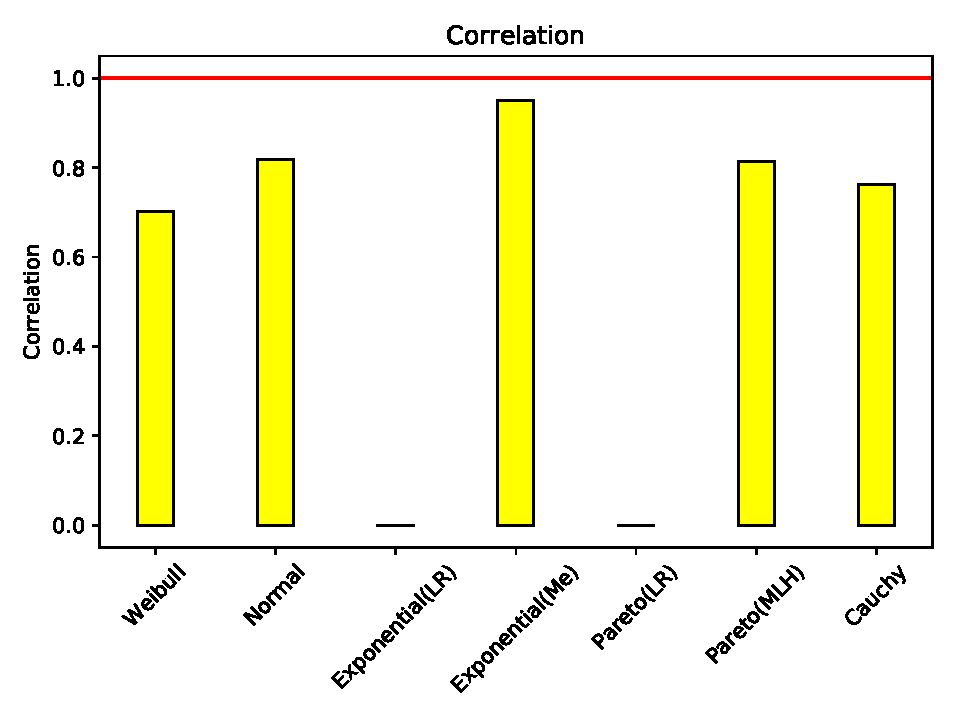
\includegraphics[width=60mm]{figures/ch4/Wan_Correlation}
        \label{Wan-correlation-skype}
    }
    \hspace{0mm}
    \subfloat[Hust Exponent]{
        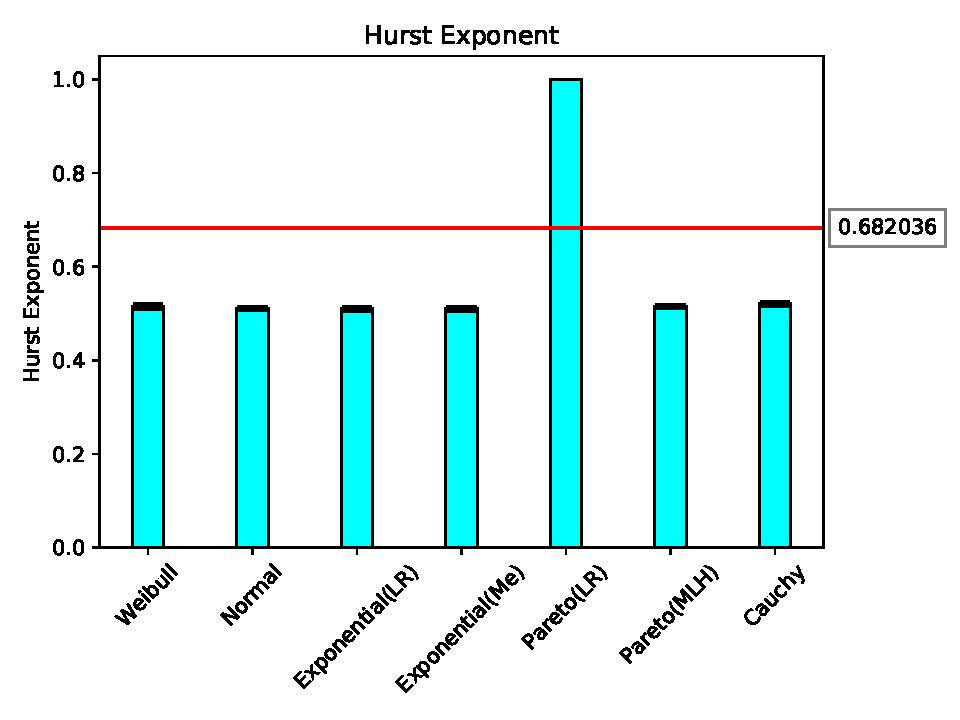
\includegraphics[width=60mm]{figures/ch4/Wan_Hurst_Exponent}
        \label{Wan-hurst-skype}
    }
    \hspace{0mm}
    \subfloat[Mean]{
        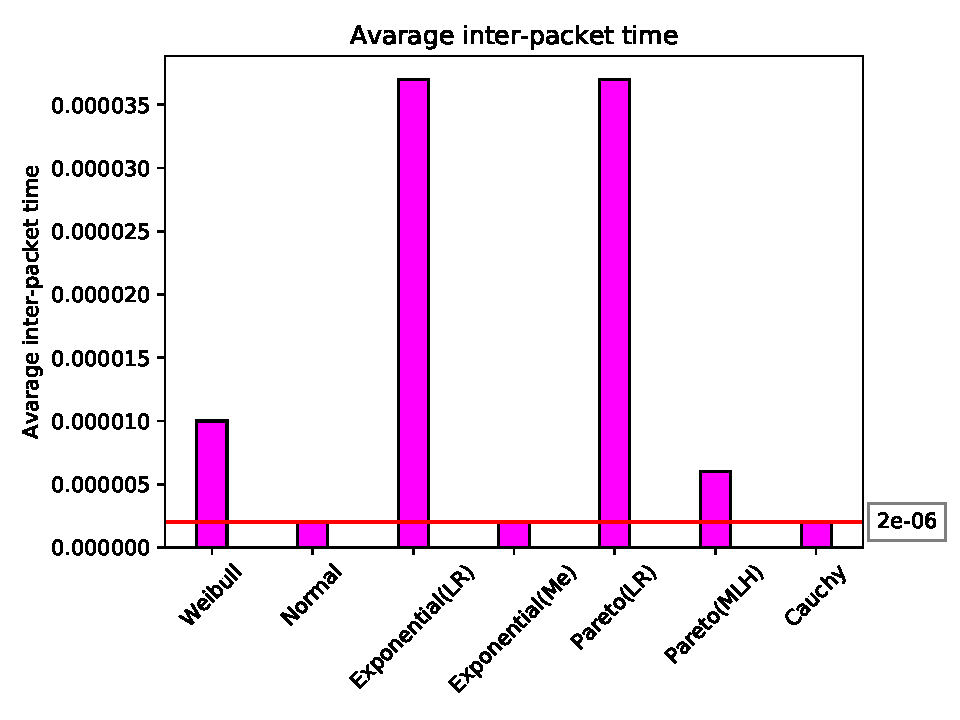
\includegraphics[width=60mm]{figures/ch4/Wan_Mean}
        \label{Wan-mean-skype}
    }
    \hspace{0mm}
    \subfloat[Standard Deviation]{
        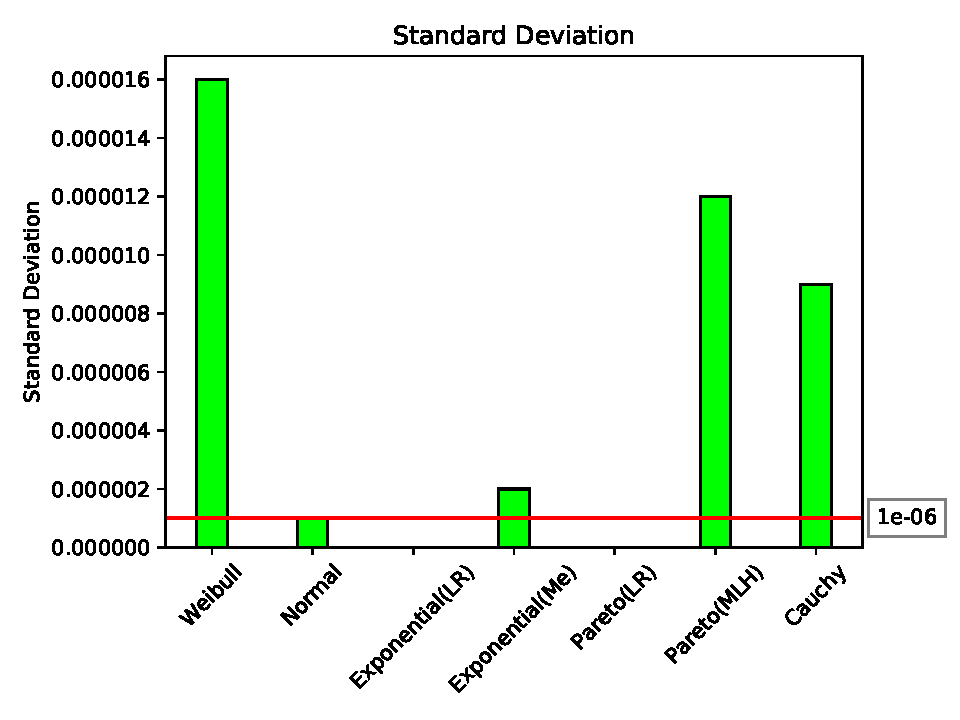
\includegraphics[width=60mm]{figures/ch4/Wan_Standard_Deviation}
        \label{Wan-std-skype}
    }
    \caption{Statistical parameters of \textit{wan-pcap} and its approximations}
    \label{fig:correlation-hurst-wan-pcap}
\end{figure}
\end{figure}


\begin{figure}[ph]
%%%%%%%%%%%%%%%%%%%%%%%
% AIC BIC  diff
%%%%%%%%%%%%%%%%%%%%%%%
\begin{table}[H]
\centering
\caption{Relative difference(\%) between $AIC$ and $BIC$.}
\scalebox{0.90}{ 
\begin{tabular}{ccccc}
\hline
                & skype-pcap & \begin{tabular}[c]{@{}l@{}}lan-gateway\\ -pcap\end{tabular} & wan-pcap & \begin{tabular}[c]{@{}l@{}}lan-firewall\\ -pcap\end{tabular} \\ \hline
Weibull         & $7.47E-01$   & $3.96E-04$                                                    & $8.86E-05$ & $9.21E-04$                                                     \\
Normal          & $7.04E-01$   & $4.66E-04$                                                    & $7.58E-05$ & $NaN$                                                          \\
Exponential(LR) & $9.54E+00$   & $2.97E-04$                                                    & $4.26E-05$ & $2.81E-03$                                                     \\
Exponential(Me) & $2.00E+00$   & $2.00E-04$                                                    & $3.68E-05$ & $6.90E-04$                                                     \\
Pareto(LR)      & $2.53E-01$   & $4.25E-04$                                                    & $5.36E-05$ & $1.13E-03$                                                     \\
Pareto(MLH)     & $4.45E+00$   & $4.25E-04$                                                    & $7.74E-05$ & $1.04E-03$                                                     \\
Cauchy          & $1.23E-01$   & $5.97E-04$                                                    & $8.08E-05$ & $8.90E-03$                                                     \\ \hline
\end{tabular}
}
\label{tab:aic-bic-diff}
\end{table}
%%%%%%%%%%%%%%%%%%%%%%%
%validation Cost function
%%%%%%%%%%%%%%%%%%%%%%%
\begin{figure}[H]
    \centering
    \subfloat[\textit{skype-pcap}]{
        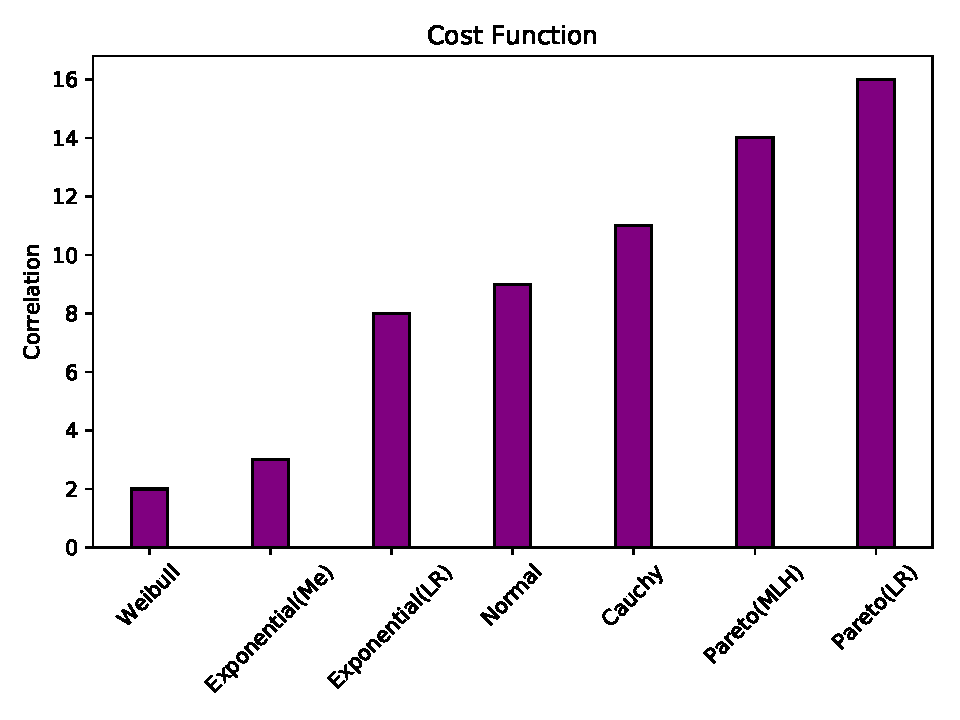
\includegraphics[width=62mm]{figures/ch4/Skype_costFunction}
        \label{cost-skype-pcap}
    }
    \hspace{0mm}
    \subfloat[\textit{lan-gateway-pcap}]{
        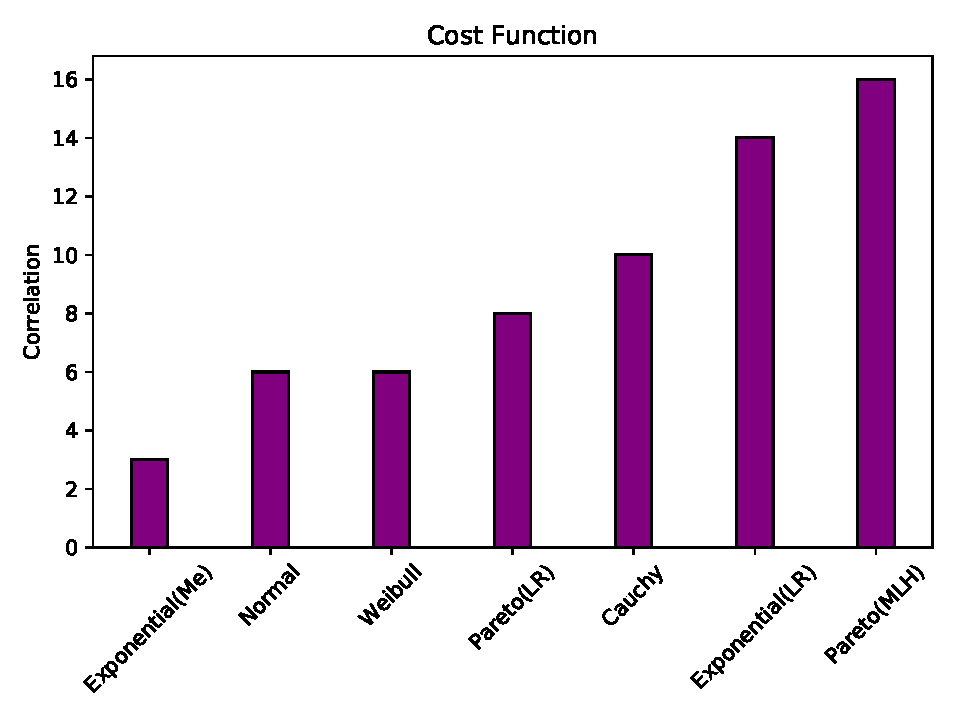
\includegraphics[width=62mm]{figures/ch4/bigFlows_costFunction}
        \label{cost-lan-gateway-pcap}
    }
    \hspace{0mm}
    \subfloat[\textit{lan-firewall-pcap}]{
        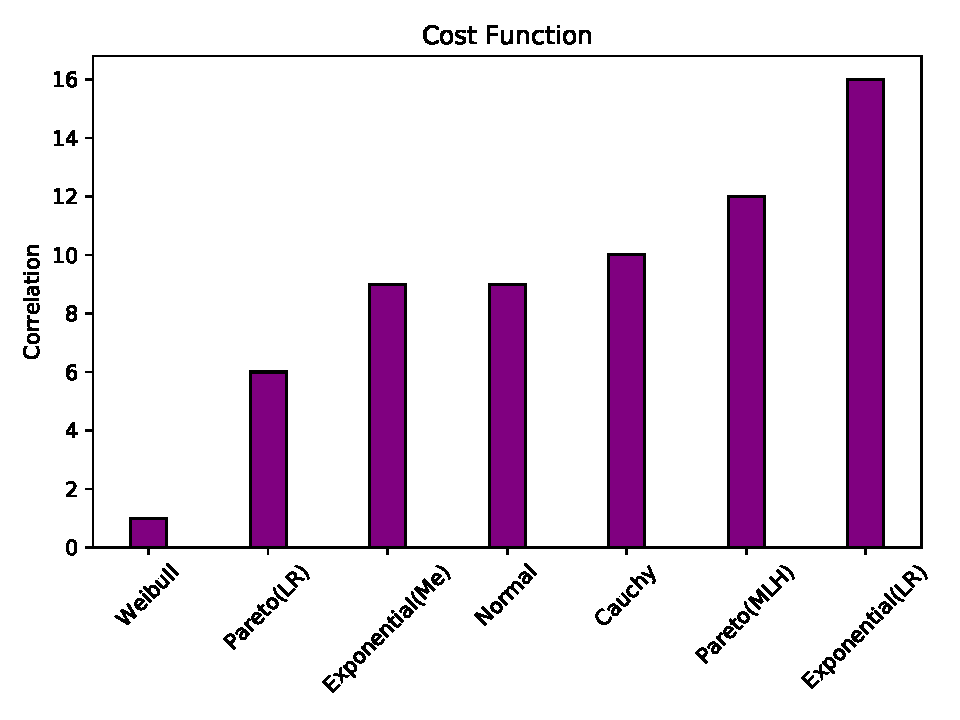
\includegraphics[width=62mm]{figures/ch4/Lan_costFunction}
        \label{cost-lan-pcap}
    }
    \hspace{0mm}
    \subfloat[\textit{wan-pcap}]{
        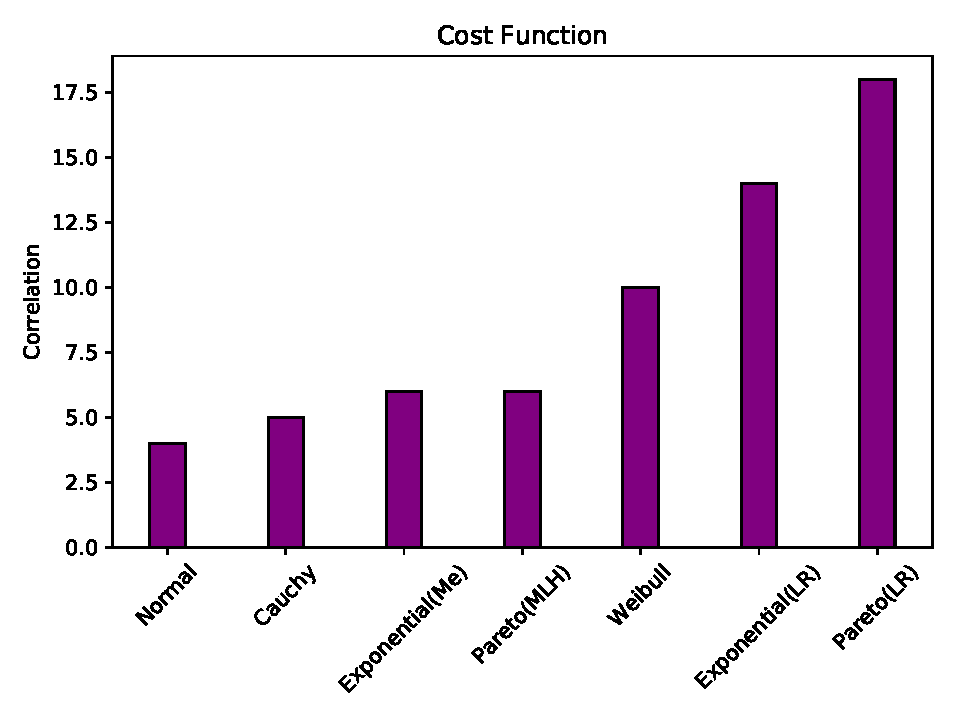
\includegraphics[width=62mm]{figures/ch4/Wan_costFunction}
        \label{cost-wan-pcap}
    }
    \caption{Cost function $J_M$ for each one of the data-sets used in this validation process}
    \label{fig:cost-function}
\end{figure}
\end{figure}

\begin{figure}[!ht]
%%%%%%%%%%%%%%%%%%%%%%%
% AIC / BIC order
%%%%%%%%%%%%%%%%%%%%%%%
\begin{figure}[H]
    \centering
    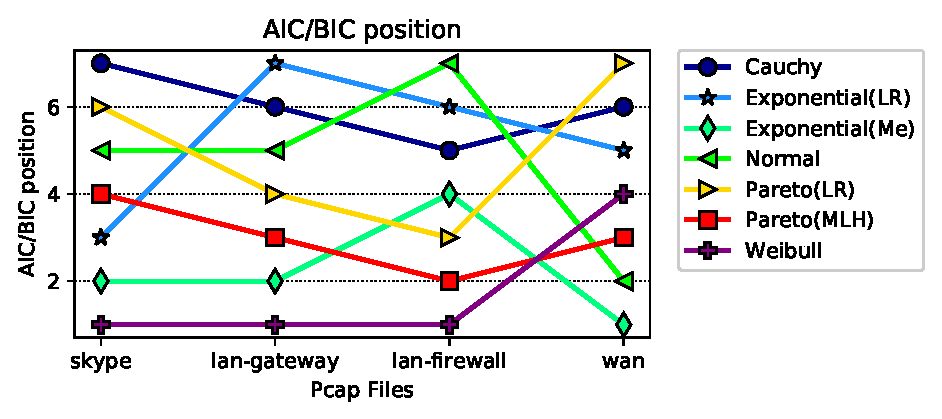
\includegraphics[scale=0.8]{figures/ch4/aic-bic-order.eps}
    \caption{Comparision of the quality order of each model given by $AIC$ and $BIC$}
    \label{fig:aic-bic-order}
\end{figure}
%%%%%%%%%%%%%%%%%%%%%%%
% Cost function order
%%%%%%%%%%%%%%%%%%%%%%%
\begin{figure}[H]
\centering
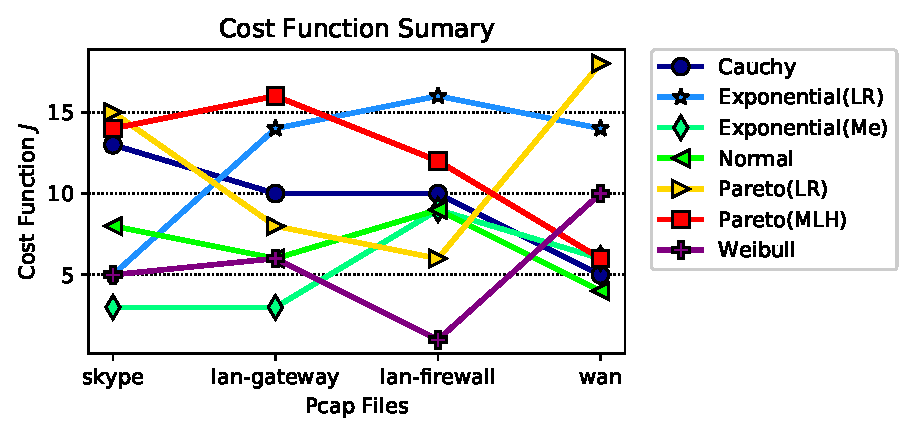
\includegraphics[scale=0.8]{figures/ch4/cost-function-summary.eps}
\caption{$J_M$ for each one of the datasets used in this validation process.}
\label{fig:model-order-cost}
\end{figure}
\end{figure}


\begin{figure}[!ht]
%%%%%%%%%%%%%%%%%%%%%%%
% CDFs eample
%%%%%%%%%%%%%%%%%%%%%%%
\begin{figure}[H]
\centering
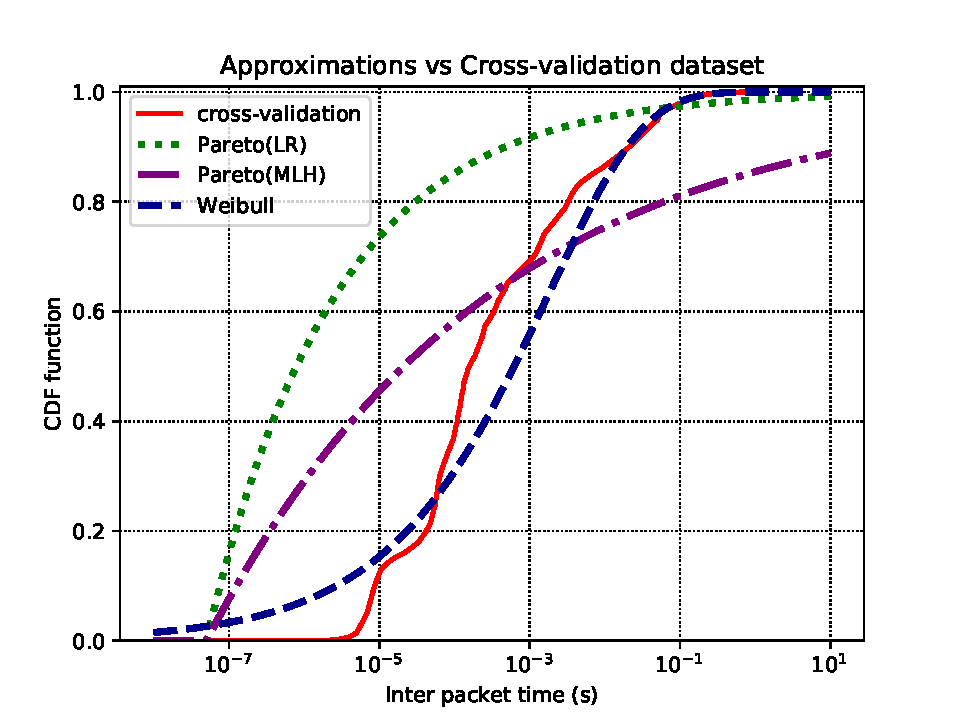
\includegraphics[scale=0.7]{figures/ch4/cdfs}
\caption{Inter-packet times CDF function and stochastic models for \textit{firewall-pacap}.}
\label{fig:lan-firewall-cdf}
\end{figure}
%%%%%%%%%%%%%%%%%%%%%%%
% relative diff
%%%%%%%%%%%%%%%%%%%%%%%
\begin{figure}[H]
\centering
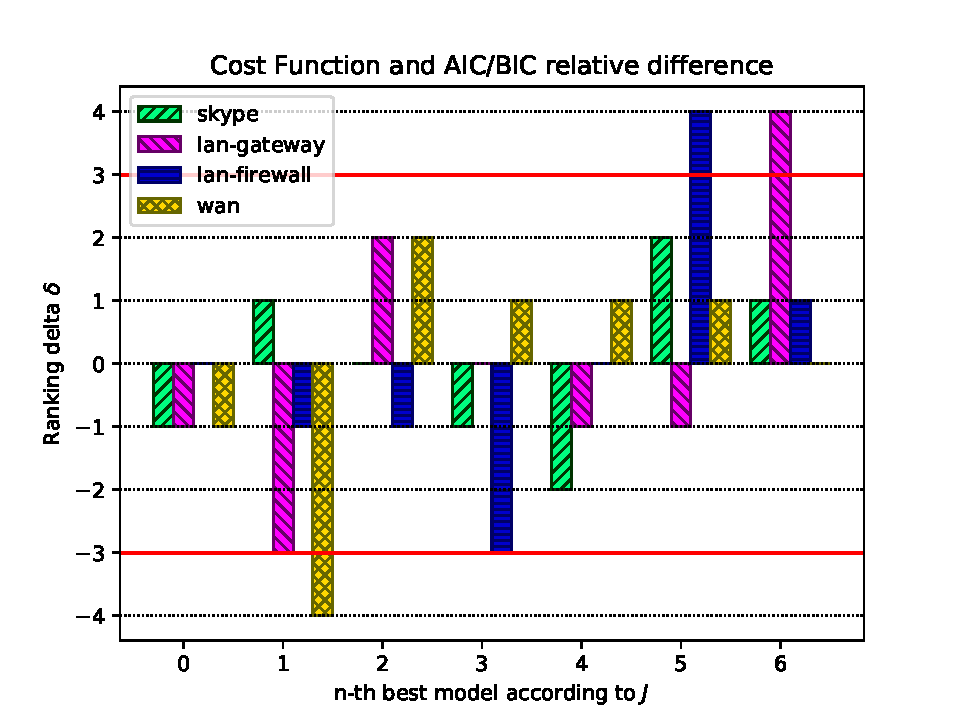
\includegraphics[scale=0.75]{figures/ch4/aicbic-costfunction-relative-diff}
\caption{Comparison of the model selection order for $BIC$/$AIC$ and  $J_M$ for each \textit{pcap}.}
\label{fig:cost-function_vs_aic-bic}
\end{figure}
\end{figure}


Here in this chapter we only discuss the approximation and QQplots achieved obtained by the \textit{pcap} \textit{skype-pcap}. All the other comments will be referent to the general results. The other fitting and QQ plots are provided on appendix~\ref{ap:aditional-plots} as a reference. 
We divided our analysis into 5 steps:
\begin{enumerate}
    \item \textit{CDF plots}
    \item \textit{QQplots}
    \item \textit{AIC} and \textit{BIC}
    \item \textit{Correlation, Hurst Exponent, Mean, and Standard Deviation} 
    \item  \textit{AIC} and \textit{BIC} vs. $\boldsymbol{J_M}$ 
\end{enumerate} 

\smallskip \noindent \textbf{\textit{CDF plots}}

Figure~\ref{fig:aproximation-original-cdf}  shows the CDF plots for \textit{skype-pcap}. They are on log-scale, which provide a better visualization for small time scales. 

\begin{itemize}
    \item We initially expected a good performance of heavy-tailed processes, but it depended on each case.
    \item Visually, the best result have seemed to be
    the Weibull trough linear regression, followed by Exponential(Me) -- what the $AIC$/$BIC$ analysis (figure~\ref{fig:aic-bic-order}) have confirmed. Also, Figure~\ref{fig:correlation-hurst-skype-pcap} show Weibull having the best Correlation and Hurst exponent, and the third best mean; while Exponential(Me) have had the best mean and the second best Correlation and Hurst exponent. 
    \item The Cauchy process have imposed an almost constant traffic, with the average inter-packet time close to the mean. Figure~\ref{fig:correlation-hurst-skype-pcap} confirms this observation since the process standard deviation is small, and the mean inter-packet time is close to the original (the second best);
    \item Exponential processes did not represented well small and larger values, compared to heavy-tailed processes, but were good to describe values closer to the average. On the other hand, a self-similar processes, such as Weibull and Pareto, have had a higher dispersion. The random-generated values were more wide-spared over the time -- what did not necessarily have implied on quality, as we are going to see. For example, Pareto(MLH) tended to over-estimate the amount of long values of inter-packet times, having a slower convergence of the CDF to one compared to the other processes -- about 20\% of the values are larger than 10 seconds. Cauchy for most of the case as a good process to represent the mean inter-packet times, but did no performed so well on other metrics (Figures      ~\ref{fig:correlation-hurst-wan-pcap}, ~\ref{fig:correlation-hurst-Lan-pcap}, ~\ref{fig:correlation-hurst-lan-gateway-pcap}, and  ~\ref{fig:correlation-hurst-skype-pcap})
    \item For the normal process, all values smaller than zero were zeroed, what have caused a vertical "off-set" on its CDF distribution. 
\end{itemize}

\smallskip  \noindent  \textbf{\textit{QQplots}}

On the QQplots(figure~\ref{fig:qq-skype}) we have observed that the original data had a much more influential heavy-tail effect when compared to the randomly generated on Cauchy, Exponential(Me), Pareto(LR), and Pareto(MLH) (appendix~\ref{ap:revision-probability}). We can observe  the The original data(samples) had a much influential heavy-tail effect compared to  the estimated data. We  verified this by the almost horizontal line made of blue dot-marks. On the other hand, Weibull process have had a much similar \textit{QQplot} compared to the samples.
Also we can identify a right-skew for Exponential(LR), Exponential(Me) and Pareto(MLH), and a left-skew for Cauchy, Pareto(LR) and Weibull.  On the other hand, the Normal distribution have presented a bi-modal behavior -- The first mode is on zero (since we zeroed all values smaller than zero), and the second, is close to the the average.


\smallskip \noindent  \textbf{\textit{AIC} and \textit{BIC}}

The calculated values for $AIC$, $BIC$, and processes parameters for all the traces are in table~\ref{tab:prototype-results}. We have verified in all cases  that the difference between $BIC$ and $AIC$ for a given process was always smaller compared to the difference between the values of a same criteria but among different processes to represent the same traffic. In another words, changing the criteria matter less than changing the process distribution. In our study,  $AIC$ and $BIC$ always have pointed to the same model ordering (figure ~\ref{fig:aic-bic-order}).

To compare these values of the information criteria, we calculated on the table  table~\ref{tab:aic-bic-diff} the relative difference between $AIC$ and $BIC$\footnote{ 
To calculate the relative difference $r_\%$ shown on table~\ref{tab:aic-bic-diff} we used this formula:
\begin{equation}
    r_\% = \frac{|V_1-V_2|}{\frac{(V_1+V_2)}{2}}\cdot100 
\end{equation}
}. The table indicate that the $AIC$ and $BIC$ converged to a common value as  the dataset size increasead\footnote{from the small to the larger dataset we have \textit{skype-pcap}, \textit{lan-gateway-pcap}, \textit{wan-pcap}, and \textit{lan-firewall-pcap}}. 
This result have indicated that, if the dataset is large enough, $AIC$ and $BIC$ will point to the same result. As table~\ref{tab:aic-bic-diff} shows, 9.54\% for Exponential(LR) was the larger difference between the information criteria. For the other pcaps, with a greater dataset, the differences were always small than 0.001\%. But, even the \textit{lan-firewall-pcap} being the largest one, the relative difference between its $AIC$ and $BIC$ is small than the ones form \textit{wan-pcap} and \textit{lan-gateway-pcap}. However, we have that information criteria depends on the likelihood value, and this on the individual probability of each value. We note that the standard deviation for packet times in \textit{lan-firewall-pcap} is considerably larger~\ref{fig:correlation-hurst-Lan-pcap}. This may be one of the possible causes for this observed behavior.



\smallskip \noindent  \textbf{\textit{Correlation, Hurst Exponent, Mean, and Standard Deviation}} 

In Figures ~\ref{fig:correlation-hurst-skype-pcap}, ~\ref{fig:correlation-hurst-lan-gateway-pcap}, and ~\ref{fig:correlation-hurst-wan-pcap}, and  ~\ref{fig:correlation-hurst-Lan-pcap} we show the results of properties calculated for each of the simulations of the stochastic processes: Correlation, Exponent of Hurst, Mean and Standard deviation. Each figure represents a different pcap file. The red horizontal line represents the value of the original traffic. Analyzing the quality of $AIC$ and $BIC$ on \textit{skype-pcap}, based on the figure results we see that concerning Correlation and Self-similarity it picked the right model: Weibull. Also regarding the average packet rate and dispersion, it is still one of the best choices. On regarding to the Mean, Exponential(Me) and Cauchy had the best performances. Regarding to the Standard Deviation, Exponential(Me) and Exponential(LR) had the best performance. Not by chance, Exponential(Me) $AIC$ and $BIC$ presented as the second best option. Comparing the results of the figures with the order suggested by AIC to BIC(Figure ~\ref{fig:aic-bic-order}), we noticed that the best ranked models showed a good performance in the metrics in general. We show the cost function $J_M$, able to summarize all the primary metrics in a single number, in figure~\ref{fig:cost-function}. All these results are abstracted by the cost function $J_M$. 


\smallskip \noindent  \textbf{\textit{AIC} and \textit{BIC} vs. $\boldsymbol{J_M}$ } 

Table~\ref{tab:prototype-results} summarizes the estimates obtained  for $AIC$, $BIC$, and the stochastic process estimated parameters for all \textit{pcap} traces. Each model order is graphically presented in Figure ~\ref{fig:aic-bic-order}.  For all \textit{pcap} experiments, we verify that the difference between $BIC$ and $AIC$ for a given function is always smaller than its value among different distributions. As shown in the table~\ref{tab:prototype-results}, $AIC$ and $BIC$ criteria always pointed to the same model ordering. Table~\ref{tab:aic-bic-diff} presents the percentage difference between the obtained values. We verify that their values tend to converge when the dataset increases. 

Figure~\ref{fig:cost-function} illustrates the cost function values for all the models on each \textit{pcap} file. For example, for \textit{skype-pcap}, $BIC$ and $AIC$ points that  Weibull and Exponential (Me) are the best representation for the traffic. The cost function used for cross-validation points both as best options, along with Exponential(LR).  To simplify the visualization and comparison of the differences between the rankings given by both methodologies, we created the plot~\ref{fig:cost-function_vs_aic-bic}.
The Figure~\ref{fig:cost-function_vs_aic-bic} presents a chart with the relative differences from the order of each model. Taking as a reference the position of each model given by $J$, we sorted them from the better to the worst (0 to 6, on the x-axis), and measured the position distance with the ones given by the information criteria. Since the worst case for this value is 6(opposite correspondence), we draw a line on the average: the expected value in the case no positive or negative correspondence existed between both information criteria and $J$. Using the $\phi$ operator, as defined before, we can calculate the ranking delta, as explained, for the \textit{i-th} model by:

\begin{equation}
\delta(m_i) = \phi(Jv, m_i) - \phi(IC, m_i)
\end{equation}

Where $Jv$ and $IC$ are the ordered pairs vectors on models and cost functions/information criteria, from the best to the worst, respectively.  We can observe that for mos to the use cases, the information criteria and the cost function had chosen models in a similar order. A hypothesis ranked well by one, tend to be ranked as good on the other. For the 28 possible study cases, 19 (68\%) had the same, or one-position difference on the ranking. 
Also, can point that $AIC$/$BIC$ tended to prioritize most of the heavy-tailed processes, such as Weibull and Pareto (except by Cauchy). It is a useful feature when the scaling and long-range characteristics of the traffic have to be prioritized by the selected model. 

Finally, we point out the $AIC$ and $BIC$ presented a bias in favor of Pareto(MLH). Even though it was never ranked as the best model, it was always better positioned by $AIC$ and $BIC$ than by $J$. We explain this result by the fact that $AIC$ and $BIC$ calculation uses the model likelihood, and the  Pareto(MLH) maximizes it.  This effect is clear on the \textit{lan-firewall-pcap}. On the figure~\ref{fig:lan-firewall-cdf} we plot the cross-validation dataset, the best fitting pointed by both methods (Weibull), and the second-best indicated by $J$ (Pareto(LR)) and by $AIC$/$BIC$(Pareto(MLH)). Even though Pareto(MLH) has a good performance representing small values, about 10\% of the inter-packet times are higher than 10 seconds, a prohibitive high value. It makes the Pareto(LR) overhaul performance better.


\subsection{Conclusion}


In this work, we introduce and evaluate a method based on $BIC$ and $AIC$ for analytic selection criteria of the best stochastic process to model network traffic. We use a cross-validation methodology based on random data generation following the selected models and cost function measurements. We observe that both $AIC$ or $BIC$ and the cost function were able to pick the first models in the same order, corroborating to our hypothesis of Akaike and Bayesian information criteria as reliable model selectors for network inter-packet times. We can conclude that $BIC$ and $AIC$ are suitable alternatives to derive realistic network traffic models for synthetic traffic generation. The only cave we point is on the use of the Maximum Likelihood method, that can over-prioritized some models over others with better performance. We summarize the implementation used on SIMITAR on algorithm~\ref{alg:stochasticModelFitting}.

%%%%%%%%%%%%%%%%%%%%%%%%%%%%%%%%%%%%%%%%%%%%%%%%%%%%%%%%%%%%%%%%%%%%%%%%%%%%%%%
%% ALGORITHM stochasticModelFitting
\begin{algorithm}[ht!]
    \caption{stochasticModelFitting}
    \label{alg:stochasticModelFitting}
    \begin{algorithmic}[1]
        \small        \Function{stochasticModelFitting}{$interArrivalData, criterion$}
        \State $m = interArrivalData.size$
        \State $interArrivalData = interArrivalData + MIN\_TIME$
        \If{$m < MINIMUM\_AMOUNT\_OF\_PACKETS$}
        \State $model\_list = \{constant\}$
        \Else
        \State $model\_list = \{weibull, pareto\_lr, pareto\_mlh, exponential\_me, exponential\_lr, normal,$
        \State $cauchy, constant\}$
        \EndIf
        
        \For{$model$ \textbf{in} $model\_list$}
        \State $model.fitting\_model(interArrivalData)$
        \EndFor
        \State $model\_list.sort(criterion)$
        \State \textbf{return} $model\_list$
        \EndFunction
    \end{algorithmic}
\end{algorithm}



\section{\texttt{calcOnOff}: an algorithm for estimating flow packet-train periods}


As we discussed in chapter~\ref{ch:architecture},  we developed an algorithm we call \texttt{calcOnOff}, listed on algorithm~\ref{alg:calcOnOff}. This procedure estimates the sizes of packet trains, as periods between packet trains in a flow context. 
This procedure receives as input values:

\begin{enumerate}
\item  \textbf{\texttt{arrivalTime}}: the list of packets arrivals on time on the flow. For example, if we have five packets arriving every two seconds, we would have: \texttt{arrivalTime = [0, 2, 4,  6, 8]};
\item  \texttt{deltaTime}: the list of inter-packet times on the flow. Following the same example presented before, we would have: \texttt{deltaTime = [2, 2, 2, 2]}. 
\item  \textbf{\texttt{cutTime}}: the time threshold that defines if we are still in the same train of packets, or a new one. 
\item  \textbf{\texttt{minOnTime}}: is the minimum length of flow ON time. minOnTime were used mainly to avoid ON times of zero seconds, in the case of only one packet, or when the time between packets is smaller than the operational system precision. 
\item  \textbf{\texttt{psSizeList}}: the list of packet sizes in bytes. 
\end{enumerate}


%%%%%%%%%%%%%%%%%%%%%%%%%%%%%%%%%%%%%%%%%%%%%%%%%%%%%%%%%%%%%%%%%%%%%%%%%%%%%%%
%% ALGORITHM CALC-ON-OFF
\begin{algorithm}[pt!]
    \caption{calcOnOff}
    \label{alg:calcOnOff}
    \begin{algorithmic}[1]
        \small
        \Function{calcOnOff}{$arrivalTime, deltaTime, cutTime, minOnTime$}%\Comment{Where A - array, p - left, q - middle, r - right}
        \State $m = deltaTime.length() - 1$
        \State $j = 0$
        \State $lastOff = 0$
        \State $pktCounterSum = 0$
        \State $fileSizeSum = 0$
        \For{$i = 0:m$}
        \State $pktCounterSum = pktCounterSum + 1$
        \State $fileSizeSum = fileSizeSum + psSizeList[i, 1]$
        \If{$deltaTime[i] > cutTime$} 
        \If{$i == 1$} \Comment{if the first is session-off time}
        \State $j++$
        \State $onTimes.push(minOnTime)$
        \State $offTimes.push(deltaTime[i])$
        \State $pktCounter.push(pktCounterSum)$
        \State $fileSize.push(fileSizeSum)$
        \State $pktCounterSum = 0$
        \State $fileSizeSum = 0$
        \Else \Comment{base case} 
        \State $pktCounter.push(pktCounterSum)$
        \State $fileSize.push(fileSizeSum)$
        \State $pktCounterSum = 0$
        \State $fileSizeSum = 0$
        \If{$j == 0$}
        \State $onTimes.push(arrivalTime[i - 1])$
        \State $offTimes.push(deltaTime[i])$
        \Else \Comment{others on times} 
        \State  $onTimes.push(max(deltaTime[i-1] - deltaTime[lastOff], minOnTime))$ 
        \State  $offTimes.push(deltaTime[i])$
        \EndIf
        \State $lastOff = i$
        \EndIf 
        \EndIf       
        \EndFor
        \State $pktCounterSum = pktCounterSum + 1$
        \State $fileSizeSum = fileSizeSum + psSizeList[m]$
        \If{$lastOff == m - 1$} \Comment{ if last is session-off }
        \State $onTimes.push(minOnTime)$ % on time
        \Else \Comment{ base last case}
        \If{$lastOff \neq 0$}
        \State $onTimes.push(arrivalTime[m] - arrivalTime[lastOff])$ 
        \Else 
        \State $onTimes.push(arrivalTime[m])$ \Comment{there was just on time}
        \EndIf
        \EndIf
        \State $pktCounter.push(pktCounterSum)$
        \State $fileSize.push(fileSizeSum)$
        \State \textbf{return} $onTimes, offTimes, pktCounter, fileSize$
        \EndFunction
    \end{algorithmic}
\end{algorithm}


For example, suppose a list of arrival times: 


\texttt{arrivalTime  = [0.0, 0.3  0.5, 0.6, 4.0, 4.3, 4.4 , 10.0] }

We would have the follow list of inter-packet times: 

\texttt{deltaTime = [0.3, 0.2, 0.1, 3.4,  0.3, 0.1, 5.6]}

Suppose the list of packet sizes is:

\texttt{psSizeList = [10, 20, 10, 30, 10, 40, 10, 50]}


With a \texttt{minOnTime} of 0.1 and a \texttt{cutTime} of 3 seconds, we would have the following output:

\texttt{onTimes = [0.6, 0.4, 0.1]}

\texttt{offTimes  = [3.4, 5.6]}

\texttt{pktCounter  = [4, 3, 1]}

\texttt{fileSize  = [70, 60, 50]}

Figure~\ref{fig:on-off} shows the same example, but with a text visualization, to simplify the visualization of the grouped data.

\begin{figure}
    \centering
    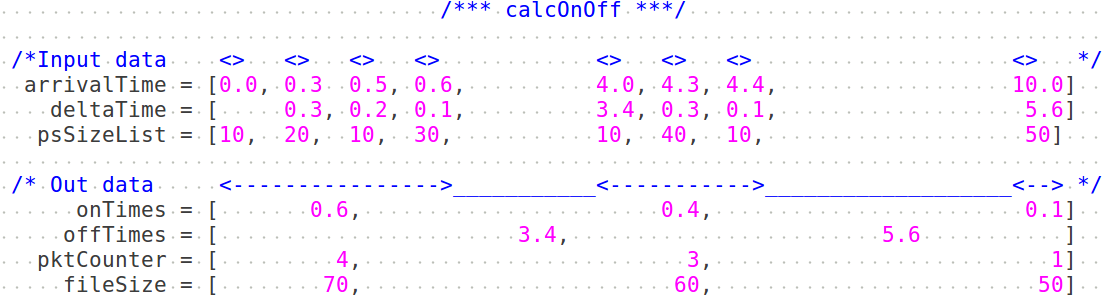
\includegraphics[width=\linewidth]{figures/ch4/on-off}
    \caption{Textual representation of the input and output data of calcOnOff.}
    \label{fig:on-off}
\end{figure}


\section{Typical header fields by Application protocols}


We also developed a simple test to guess the application protocol, based on the port numbers and the transport protocol used by each flow. If a flow matches the port number, and the transport protocol, it matches an application protocol, following the rules on table~\ref{tab:application-protocols}. 


\begin{table}[ht!]
    \centering
    \caption{Application match table}
    \label{tab:application-protocols}
    \begin{tabular}{lll}
        \hline
        Application Protocol & Transport Protocols & Transport Ports \\ \hline
        \acrshort{HTTPS}               & TCP                & 443             \\
        FTP                 & TCP                & 20, 21          \\
        HTTP                & TCP                & 80              \\
        \acrshort{BGP}                 & TCP                & 179             \\
        \acrshort{DHCP}                & UDP                & 67, 68          \\
        \acrshort{SNMP}                & UDP, TCP           & 161             \\
        \acrshort{DNS}                 & UDP, TCP           & 53              \\
        \acrshort{SSH}                 & UDP, TCP           & 22              \\
        Telnet              & UDP, TCP           & 23              \\
        \acrshort{TACACS}              & UDP, TCP           & 49              \\ \hline
    \end{tabular}
\end{table}


\section{Conclusions}


In this section, we explained on details methods mentioned in chapter~\ref{ch:architecture}. 
In this first section,  we revisited some classical works on modeling inter-packet times and packet trains. 

On the second we proposed the use of information criteria ($AIC$ and $BIC$) as tools for automatic selection of stochastic processes for inter-packet times. Since information criteria have not been tested for our study-case yet, were never tested for our study case, we developed an independent cross-validation method, based on traditional metrics for traffic validation. Since both procedures have converged to similar results, we conclude that $AIC$ and $BIC$ are reliable tools. However, we have to pay attention to processes parameterized the maximum likelihood method, since they tend to be prioritized, even performing poorly.  We abstracted this method for automatically select stochastic processes in algorithm~\ref{alg:stochasticModelFitting}. 

In the third and fourth section, we also present the methods used to estimate packet trains periods (algorithm~\ref{alg:calcOnOff}) and make the application classification (table~\ref{tab:application-protocols}). 
